%!TeX root = Chapter_Method2
\documentclass[../../CompleteThesis2/Complete_2ndDraft]{subfiles}
%\graphicspath{{../../Figures/}}
\begin{document}

This chapter presents the final method and algorithm used to obtain an estimate of the optimal diffusion length, $\sigma$, for the depth sections under consideration. It consists specifically of two sections, one presenting a walk through of the constrained optimization $\sigma$ estimation method, Section \ref{Sec:Method_SigmaMethod}, and one containing a number of tests to examine the behaviour and stability of the method and algorithm, \ref{Sec:Method_TestStab}. Finally, a discussion of the further work that could be done to improve on the method is presented in Section \ref{Sec:Method_Upgrades}.
\minitoc 

\section[$\sigma$ Estimation Method][$\sigma$ Estimation Method]{$\sigma$ Estimation Method}
\label{Sec:Method_SigmaMethod}
\begin{marginfigure}
	\centering
	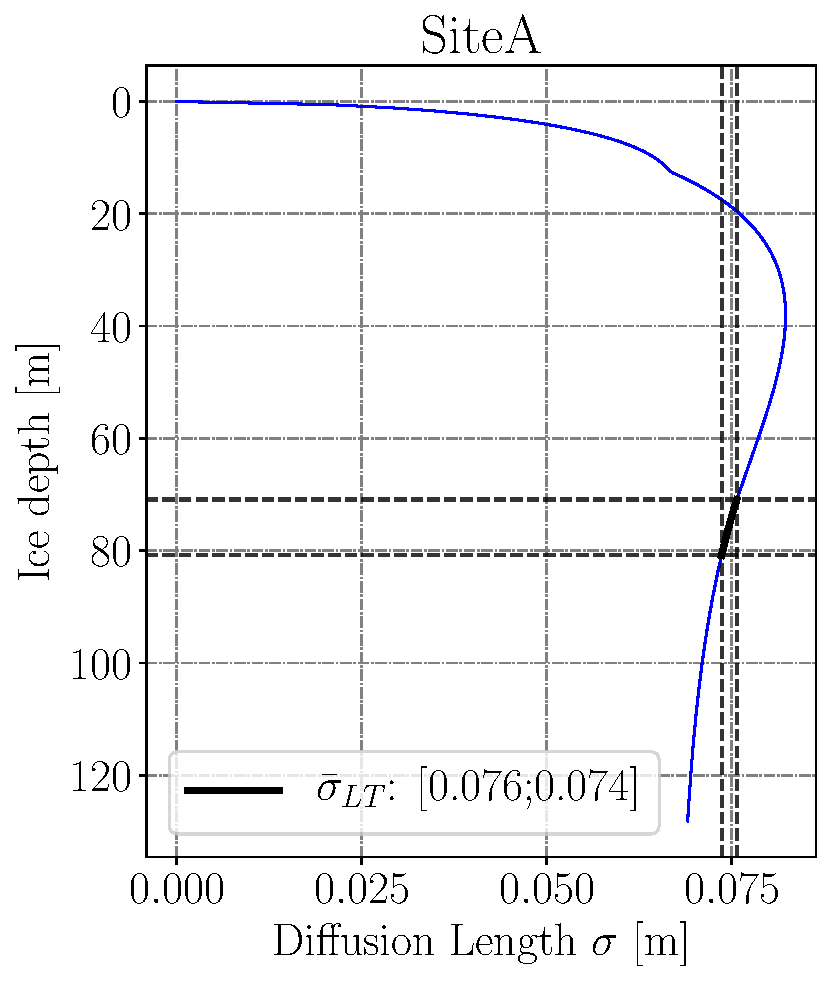
\includegraphics[width=\marginparwidth]{SiteA_DiffProf_Sigz.pdf}
	\caption[Diffusion length profile, LT]{\footnotesize Diffusion length profile with section between Laki and Tambora highlighted.}
	\label{Fig:METH_SiteA_DiffProf_Sigz}
\end{marginfigure}
As mentioned earlier, the diffusion length varies with depth, see Figure \ref{Fig:METH_SiteA_DiffProf_Sigz} for a modelled diffusion length profile for conditions at ice core drill site A. Though for the most of the final results, an assumption is made that the diffusion length along the depth section under consideration is constant, $\sigma(z)=\sigma$. This assumption is made based on the relatively small variation in diffusion length at the depths analyzed, especially compared to the uncertainty given on the final diffusion length estimates. Though this assumption is made, the subject of including a varying $\sigma(z)$ in the final analysis is presented and discussed.

%Usually, when back-diffusing a depth series, some amplitude is regained on the signal, and some peaks and troughs, that might have been washed out from the diffusion might emerge when restoring the signal. These two properties thus makes it possible to connect the diffusion length to the years counted in that section (i.e. the number of peaks and troughs). Due to the knowledge of time passed from the Laki to the Tambora event, the data, along with the restoration techniques, permits a further investigation of the diffusion length in the given section. Thus, when back-diffusing, instead of just using the diffusion length estimate from the spectra, it is possible to examine which diffusion length that results in the correct number of years counted in that section. This property is what will be utilized in the following section, which focuses on finding the optimal diffusion length of a given section.

The general idea of the optimal $\sigma$ estimation method is to back diffuse a depth series defined on an interval where the time span (i.e. the number of peaks and troughs expected in that section) is known. This allows us to use the diffusion length as a tuning parameter, to find the diffusion length estimate which generates the right number of peaks and troughs and fulfills the imposed constraints in the back diffused depth series. If more than one diffusion length meet these constraints, the largest diffusion length to still fulfill the constraints is sought after. This diffusion length is then assumed to be the optimal guess on the diffusion length in that interval, which allows for a temperature estimate, following the temperature dependence of the diffusion length, as described in Chapter \ref{Chap:IceTheory}.

The algorithm consists of two modules, where one module describes the numerical back diffusion, given an inputted depth series, core specification and specific $\sigma_0$ estimate (which is either manually inputted or estimated from the spectral analysis). The flowchart describing the processes carried out in this module can be seen in Figure \ref{Fig:FlowchartBackDiffusion}. Many of the sections in this module are only necessary in the initialization of the algorithm as these parts do not change if the inputted diffusion length estimate is changed. In Figure \ref{Fig:FlowchartBackDiffusion} anything carried out above the \textit{Frequency Filters} block to the left is only computed once, and the same with anything to the right of it, except the $\sigma_0$ estimate. The density and diffusion profile calculations, the spectral analysis and the Wiener filter construction are inherent to the depth series alone, and these analyses are carried out as previously described in this thesis.

The first module could easily be used to scan the entire one dimensional $\sigma$ space linearly, and from this analysis determine the optimal $\sigma$. This was first implemented, but turned out to be very slow - of course depending on the stepping size. But to speed up the search, a direct search method was implemented.

The second module is responsible for the optimization. This module examines the parameter space containing the diffusion length estimates, and utilizes a constrained direct search method to find the optimal diffusion length estimate. This method is illustrated through a flowchart in Figure \ref{Fig:METH_Flowchart_Optimization}. 

\subsection{Module 1: Initialization and Back Diffusion}
\label{Subsec:Method_SigmaMethod_Module1}
The first module of the algorithm, containing initialization and describing the general back diffusion method, is based on many of the aspects and models presented in the previous Chapters \ref{Chap:IceTheory} and \ref{Chap:SigAnalCompMeth}. Therefore the description of this module will focus on the work flow and not so much on the specific details of each process, as these have already been presented. The different chapters and sections containing the description of the methods used are referred to in the text of Figure \ref{Fig:FlowchartBackDiffusion}.

\begin{figure}[!htb]
	\begin{tikzpicture}[node distance=1.5cm, auto]
		\node(start) [startstop] {START};
		%----------------------------------------------------%
		\node(in1) [io, left of=start, xshift=-2.9cm, text width=4cm, align=center] {Measured depth series, $d(t)$};
		\node(empty1) [below of=in1, yshift=0.12cm] {};
		\node(empty2) [below of=in1, xshift=-0.15cm] {};
		%		\node(in1pro1) [process, below of=in1, yshift=-0.5cm] {Spline interpolation};
		\node(in1pro2) [process, below of=in1, yshift=-2cm] {Spectral analysis of $\tilde{d}(f)$};
		\node(decSpec1) [decision, below of=in1pro2, scale = 0.8, align=center] {DCT ?\\(Interpolation)};
		\node(decSpec2) [decision, left of=decSpec1, scale=0.8, xshift = -1.2cm, align=center] {FFT ?\\(Interpolation)};
		\node(decSpec3) [decision, right of=decSpec1, scale=0.8, xshift = 0.8cm] {NDCT ?};
		
		\node(in1pro3) [process, below of=decSpec1, text width=4cm, align=center] {Construct Wiener filter, $\tilde{F}(f)$};
		
		\draw[arrow] (in1) -- (start);
		\draw[-] (start) |- (empty2);
		\draw[arrow] (empty1) -- (in1pro2);
		%		\draw[arrow] (in1pro1) -- (in1pro2);
		\draw[arrow] (in1pro2) -- (decSpec1);
		\draw[arrow] (in1pro2) -- (decSpec2);
		\draw[arrow] (in1pro2) -- (decSpec3);
		\draw[arrow] (decSpec1) -- (in1pro3);
		\draw[arrow] (decSpec2) -- (in1pro3);
		\draw[arrow] (decSpec3) -- (in1pro3);
		%	\draw[arrow] (in1pro3) -- (in1pro4);
		
		%----------------------------------------------------%
		
		\node(in2) [io, right of=start, xshift=2.5cm] {Core specs};
		\node(in2pro1) [process, below of=in2, yshift=-0.5cm] {Density profile};
		\node(in2pro2) [process, below of=in2pro1] {Diffusion profile};
		\node(in2pro3) [process, below of=in2pro2] {$\sigma_0$\textbf{ estimate}};
		\node(decSigma1) [decision, below of=in2pro3, scale = 0.8] {$\sigma_0 = \sigma_{\text{const}}$?};
		\node(decSigma2) [decision, right of=decSigma1, scale = 0.8, xshift=0.8cm] {$\sigma_0 = \sigma(z)$?};
		\node(decSigma3) [decision, left of=decSigma1, scale = 0.8, xshift=-0.8cm] {$\sigma_0 = \sigma_{\text{input}}$?};
		\node(in2pro4) [process, below of=decSigma1, text width=4cm, align=center] {Construct Transfer Function filter, $\tilde{\mathcal{G}}(f)$};
		
		\draw[arrow] (in2) -- (start);
		\draw[arrow] (start) |- (in2pro1);
		\draw[arrow] (in2pro1) -- (in2pro2);
		\draw[arrow] (in2pro2) -- (in2pro3);
		\draw[arrow] (in2pro3) -- (decSigma1);
		\draw[arrow] (in2pro3) -- (decSigma2);
		\draw[arrow] (in2pro3) -- (decSigma3);
		\draw[arrow] (decSigma1) -- (in2pro4);
		\draw[arrow] (decSigma2) -- (in2pro4);
		\draw[arrow] (decSigma3) -- (in2pro4);
		%----------------------------------------------------%
		\node(pro0) [process, below of=start, yshift=-8.5cm, text width=4.5cm, align=center] {Frequency Filters, $\tilde{F}(f)\;\frac{1}{\tilde{\mathcal{G}}}$};
		\node(pro1) [process, below of=pro0, yshift=-0.4cm, ,align=center, text width=4cm, align=center] {\textbf{Deconvolution} $\mathcal{F}\left[\tilde{d}(f)\;\tilde{F}(f)\;\frac{1}{\tilde{\mathcal{G}}(f)}\right]$ \\(Uniform resampling)};
		\node(stop) [startstop, below of=pro1, yshift=-0.4cm] {\textbf{STOP}};
		\node(out1) [io, right of=stop, align=center, xshift=2.2cm, text width=3cm] {\footnotesize{Back diffused depth series, $D(t)$}\\ $\sigma_0$};
		%\node(out2) [io, below of=out1, align=center] {\footnotesize{$\sigma_{\text{out}}$}};
		\draw[arrow] (in1pro3) |- (pro0);
		%		\draw[arrow] (decSigma1) |- (pro0);
		%		\draw[arrow] (decSigma2) |- (pro0);
		%		\draw[arrow] (decSigma3) |- (pro0);
		\draw[arrow] (in2pro4) |- (pro0);
		\draw[arrow] (pro0) -- (pro1);
		\draw[arrow] (pro1) -- (stop);
		\draw[arrow] (stop) -- (out1);
		%\draw[arrow] (stop) |- (out2);
		
		%		\draw[arrow] (in2pro3) -| (pro0);
		
	\end{tikzpicture}
	\caption[Flowchart of initialization method]{\small Flowchart of initialization method for back diffusion of a depth series given a diffusion length estimate. For the left part of the flow, the methods used are presented in the following sections: spectral transform and analysis is presented in Section \ref{Sec:SignalAnalysis_SpectralAnalysis}, frequency filtering and deconvolution as means to back diffusion in Section \ref{Sec:SignalAnalysis_BackDiffusion}, peak detection in Section \ref{Sec:CompMeths_PeakDetection}, and spline interpolation in Section \ref{Sec:CompMeths_SplinesAndInterpolation}. For the right part of the flow, the theories and methods are presented in Section \ref{Sec:Ice_DensificationAndDiffusion}.}
	\label{Fig:FlowchartBackDiffusion}
\end{figure}

The module takes an input of a measured depth series in a given interval, $d$, and the specifications concerning the drill site and the ice core in general. From here the work flow splits in two: one route(left) analyzing the depth series, and one(right) giving an estimate of $\sigma$ at that depth, based on models.

\begin{figure}[!htb]
	\centering
	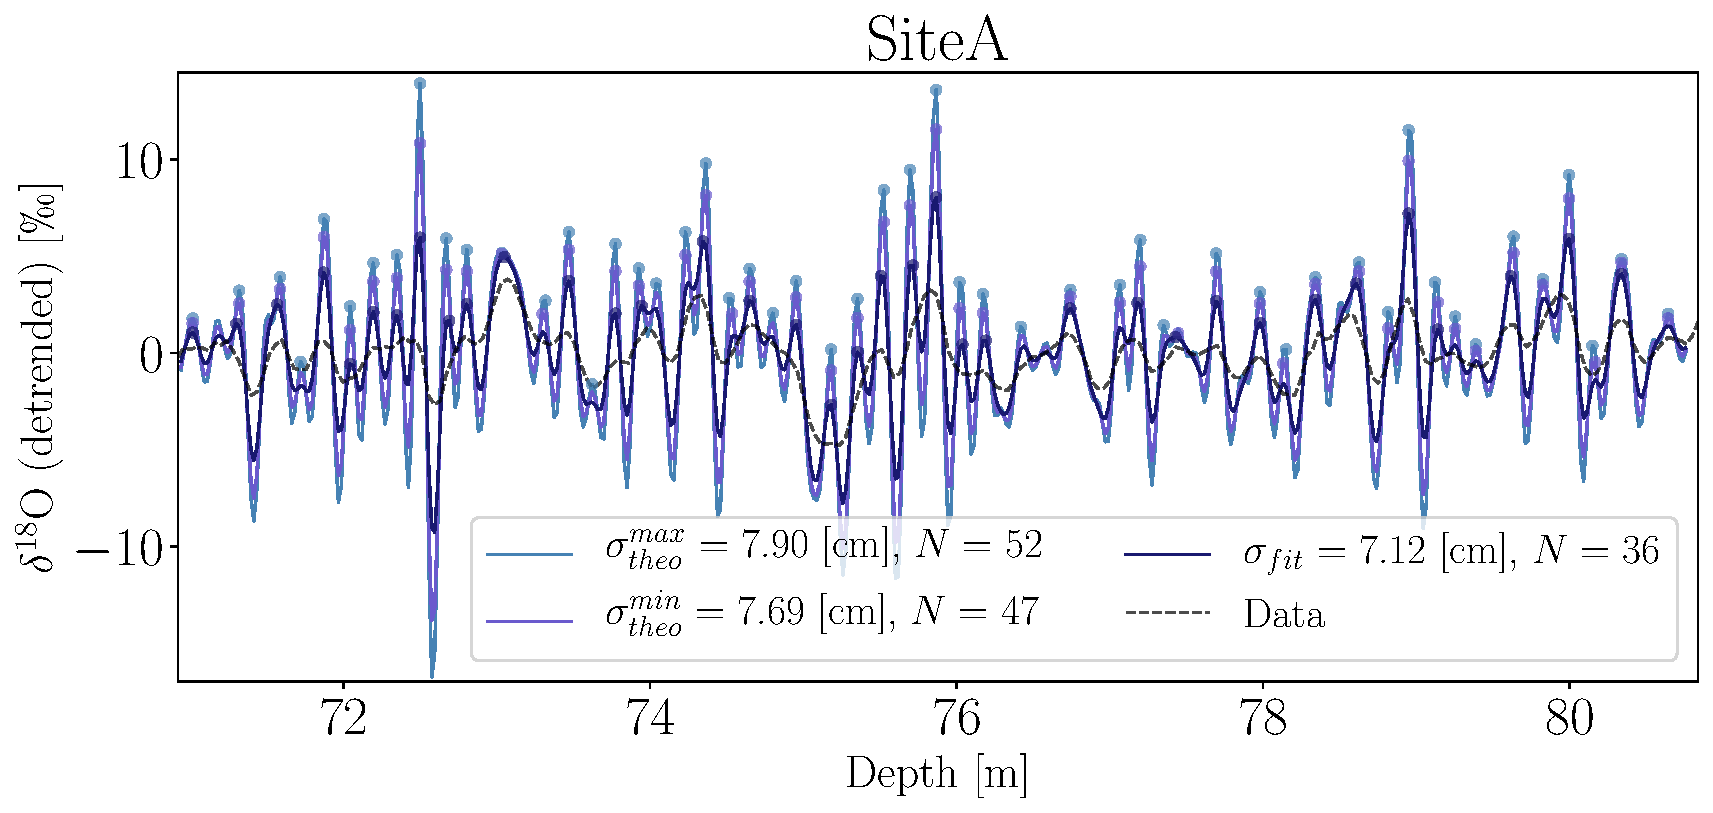
\includegraphics[width=0.95\textwidth]{SiteA_BDdata_SigmaFitSigmaTheo.pdf}
	\caption[Deconvolution with $\sigma_{\text{Theo}}$ and $\sigma_{\text{Fit}}$, Site A]{\small Backdiffused data for Site A, deconvolution with maximum and minimum $\sigma_{\text{Theo}}$, and $\sigma_{\text{Fit}}$ estimated from the PSD of the signal.}
	\label{Fig:SiteA_BDdata_SigmaFitSigmaTheo}
\end{figure}

Figures \ref{Fig:SiteA_BDdata_SigmaFitSigmaTheo} and \ref{Fig:SiteB_BDdata_SigmaFitSigmaTheo} illustrate the back diffusion with three different diffusion lengths, minimum and maximum theoretical estimate ($\sigma_{\text{Theo}}^{\text{min}}$, $\sigma_{\text{Theo}}^{\text{max}}$) and $\sigma_{\text{Fit}}$ estimated from the signal's PSD, used in the Gaussian filter. The two Figures show the difference in stability for the signal. Site A exhibits a stronger reaction to a change in $\sigma$, rapidly increasing the amplitude and number of peaks counted, whereas Site B shows smaller variation in the final restored signal.

\begin{figure}[!htb]
	\centering
	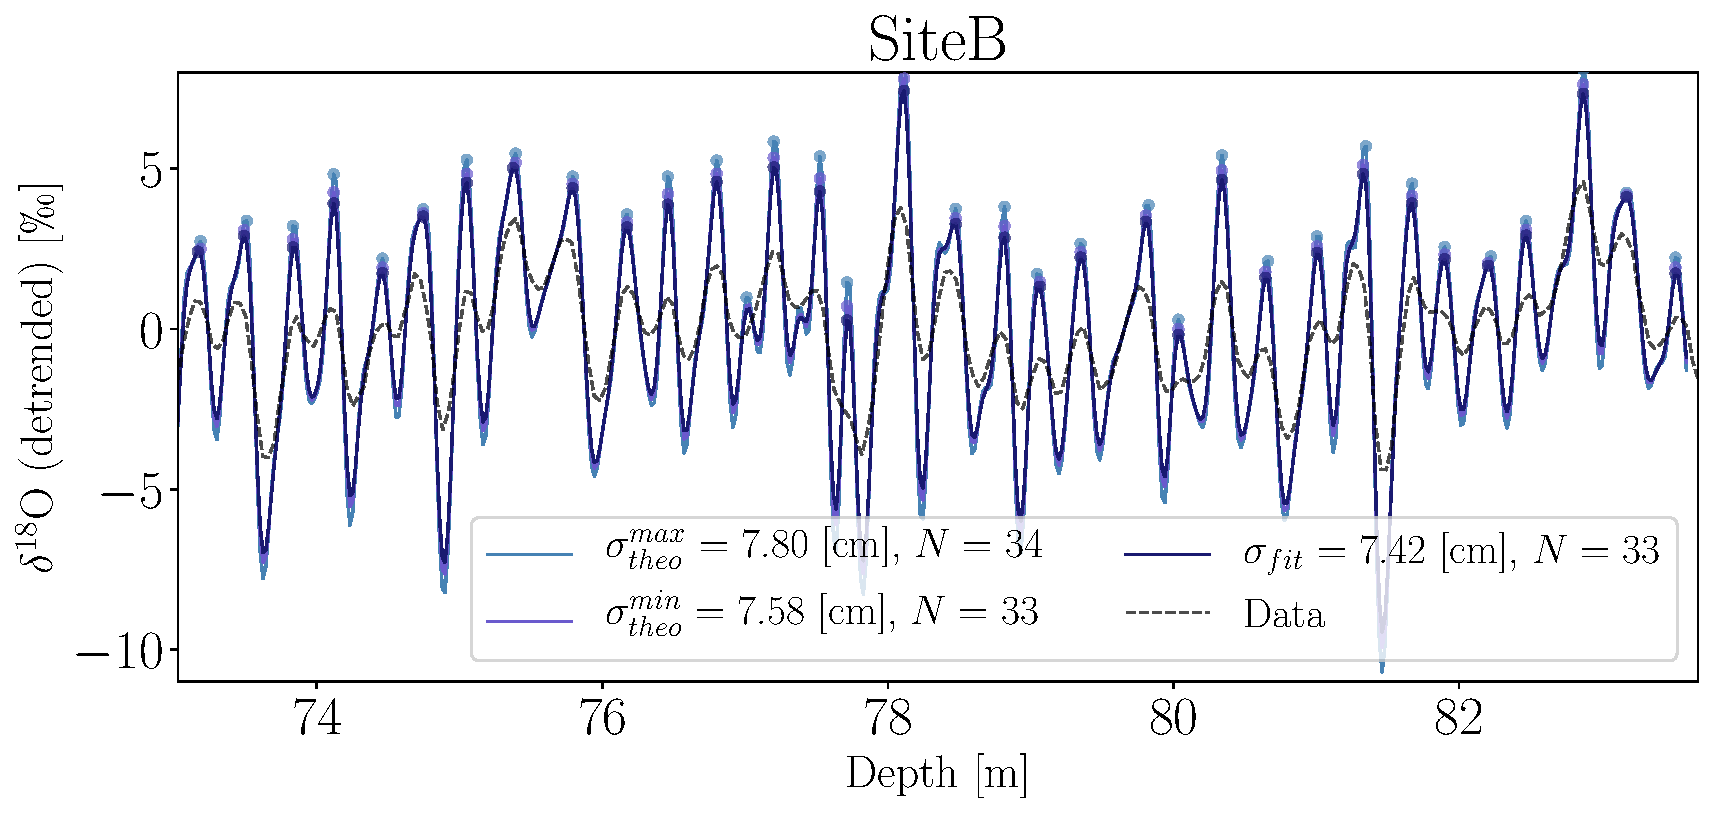
\includegraphics[width=0.95\textwidth]{SiteB_BDdata_SigmaFitSigmaTheo.pdf}
	\caption[Deconvolution with $\sigma_{\text{Theo}}$ and $\sigma_{\text{Fit}}$, Site B]{\small Backdiffused data for Site B, deconvolution with maximum and minimum $\sigma_{\text{Theo}}$, and $\sigma_{\text{Fit}}$ estimated from the PSD of the signal.}
	\label{Fig:SiteB_BDdata_SigmaFitSigmaTheo}
\end{figure}

The right flow describes how the $\sigma_0$ estimate is given on the basis of the core specifications passed into the algorithm. First, a HL-density profile is modelled, based on the necessary input parameters of annual accumulation rate $A_0$ and drill site surface temperature $T_0$, and the optional inputs of surface density $\rho_0$ and measured depth versus density data. Secondly, this density profile is used to compute a diffusion length profile, by the use of the Iso-CFM. 

The modelled diffusion length profile is then used to find a theoretical diffusion length estimate which is used as an initial guess for the diffusion length, $\sigma_0$. This is then used as the standard deviation in the Gaussian transfer function filter, $\mathcal{G}$ used for deconvolution, unless a $\sigma_0$ is inputted manually. From the modelled diffusion length profile, it is also possible to choose not just a constant $\sigma_0$, but an option for a depth-varying diffusion length, $\sigma(z)$, used in the transfer function is also available. This functionality is not analyzed in depth and would benefit from further analysis and testing.


%
%\begin{marginfigure}
%	\centering
%	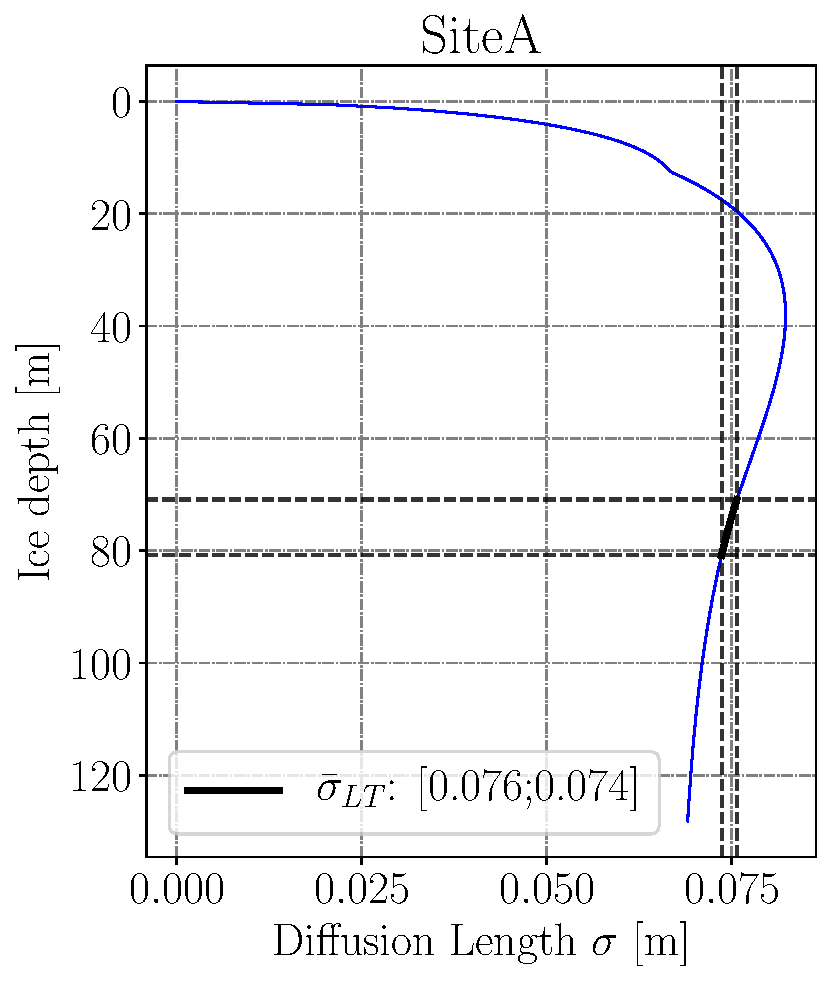
\includegraphics[width=\marginparwidth]{SiteA_DiffProf_Sigz.pdf}
%	\caption[Diffusion length profile, LT]{\footnotesize Diffusion length profile with section between Laki and Tambora highlighted.}
%	\label{Fig:SiteA_DiffProf_Sigz}
%\end{marginfigure}

If the varying $\sigma(z)$ is chosen, a fit is made to the theoretical diffusion length profile in the depth section corresponding to the Laki to Tambora depth. The back diffusion is then performed with a different Gaussian filter for each point, i.e. $\mathcal{G}(\sigma(z)) = \frac{1}{\sigma(z)\sqrt{2\pi}}\,e^{\frac{-z^2}{2\,\sigma^2}}$. $\sigma(z)$ is estimated from a fit to the theoretical diffusion length profile. In Figure \ref{Fig:METH_SiteA_DiffProf_Sigz} is shown the depth section of the diffusion length profile corresponding to that between Laki and Tambora. Figure \ref{Fig:SiteA_sigmaz_fit} shows the polynomial fit made to this depth section. 
\begin{marginfigure}
	\centering
	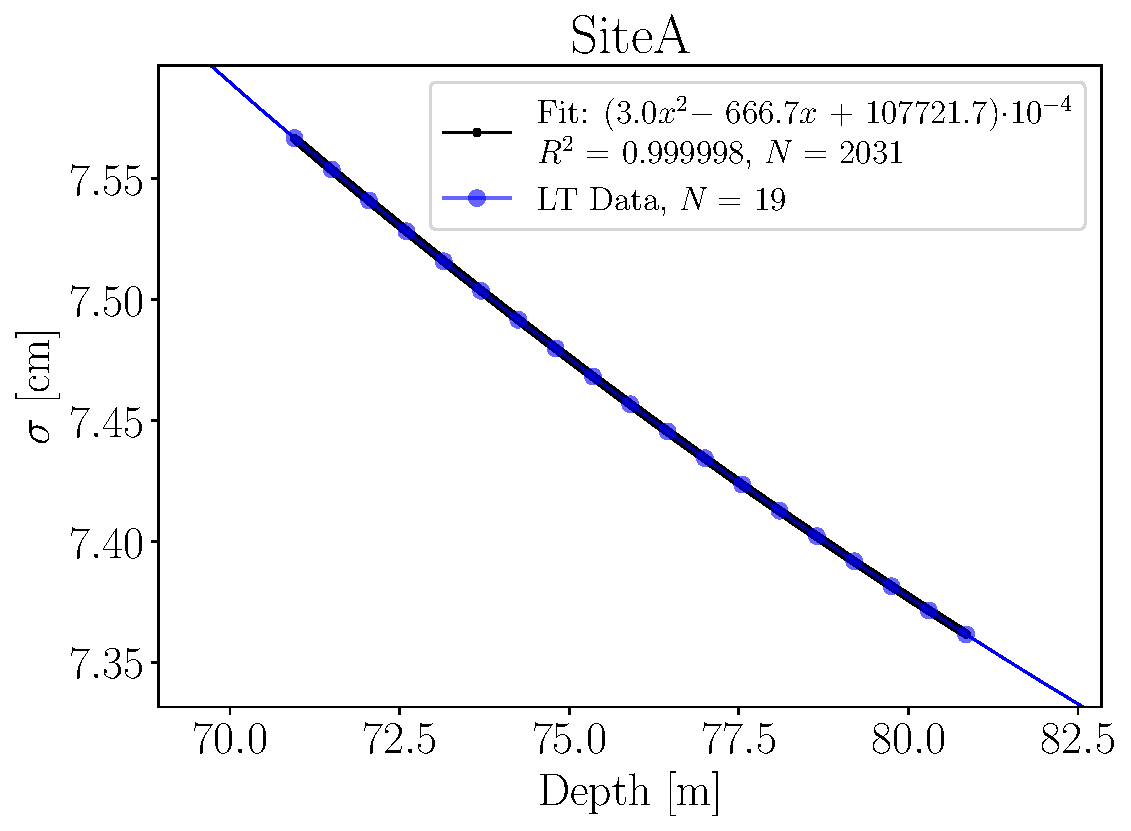
\includegraphics[width=\marginparwidth]{SiteA_sigmaz_fit.pdf}
	\caption[Diffusion length profile, fit at LT]{\footnotesize Diffusion length profile at Laki to Tambora depth, with $\sigma(z)$ fit.}
	\label{Fig:SiteA_sigmaz_fit}
\end{marginfigure}

The left flow shows the analysis carried out on the measured depth series, $d(t)$. First, the depth series is transformed to the frequency domain, with the user's choice of spectral transformation method. If FFT or DCT is chosen, the depth series will be interpolated to resemble equispaced data. Then the frequency series is analyzed according to Section \ref{Sec:SignalAnalysis_BackDiffusion}, where fits to the signal and noise are made, that again are used to construct an optimal Wiener filter, $\tilde{F}(f)$. During this process, it is optional to choose the standard deviation of the estimated noise free signal, $\sigma_{\text{tot}}$, as the diffusion length to use in the deconvolution.

Finally, the right and the left flow are combined to construct the final restoration filter, $\tilde{R}(f)=\tilde{F}(f)\,\frac{1}{\tilde{\mathcal{G}}(f)}$, which is used for optimal enhancement and restoration when deconvoluting the signal to $D(t)=\mathcal{F}\left[\tilde{d}(f)\cdot\tilde{F}(f)\cdot\frac{1}{\tilde{\mathcal{G}}(f)}\right]$, and the module returns the back diffused series $D(t)$ and the diffusion length used, $\sigma_{0}$.

\begin{figure}[!]
	\begin{tikzpicture}[node distance=1.5cm, auto]
		\node(pro1) [process, align=center] {$\sigma_0$ estimate};
		\node(in1) [io, right of=pro1, text width=2cm, align=center, xshift=3cm] {Inputs: $\Delta_{\sigma}$, $\epsilon$, $N_{\sigma}$}; 
		\node(pro2) [process, text width = 4.3cm, align=center, below of=pro1, yshift=-1.8cm] {Construct $\bar{\sigma}_0$ grid, 
			\begin{align}
				\bar{\sigma} &= \begin{bmatrix}
					\sigma_0 - \left(\frac{N_{\sigma}}{2}-1\right)\Delta_{\sigma}\\
					\vdots\\
					\sigma_0 - \Delta_{\sigma}\\
					\sigma_0 \\
					\sigma_0 + \Delta_{\sigma}\\
					\vdots \\
					\sigma_0 + \left(\frac{N_{\sigma}}{2}-1\right)\Delta_{\sigma}
				\end{bmatrix}
				\nonumber
		\end{align}};%$\bar{\sigma}=$ [$\sigma_{-2}$, $\sigma_{-1}$, $\sigma_0$, $\sigma_{1}$, $\sigma_{2}$]};
		%\node(pro3) [process, below of=pro2, text width=4.5cm, align=center, yshift=-1.5cm] {Frequency Filters, $\tilde{F}\cdot\tilde{\mathcal{G}}(\bar{\sigma})$};
		
		
		\node(pro4) [process, minimum width=5cm, minimum height = 4cm, below of=pro2, yshift=-3.3cm, align=left] {};
		\node(for1) [below of=pro4, align=left, yshift=3.cm, xshift=-1.4cm] {\textbf{for} $\sigma$ \textbf{in} $\bar{\sigma}$:};
		\node(pro4dec1) [decision, below of=pro2, text width=5cm, scale=0.9, align=left, yshift=-3cm] {
			\hspace{6mm} Deconvolution, \\ 
			\hspace{6mm} $D=\mathcal{F}\left[\tilde{d}\cdot\tilde{F}\cdot\tilde{\mathcal{G}}(\sigma)^{-1}\right]$};
		\node(empty1) [left of=pro4dec1, xshift=-2.5cm, yshift=2.8cm] {Wiener filter, $\tilde{F}$};
		\node(pro4dec2) [decision, below of=pro4dec1, text width=4cm, scale=0.9, align=left] {Count $N_{P}$ in $D$,\\ under constraints};
		\node(pro4dec3) [draw, right of=pro4dec2, fill=Gray, xshift=4cm, text width=2.5cm, scale=0.8] {\textbf{if} $N_{P} \leq 33$: \\ 
			\hspace{5mm} $P_i=0$,\\ 
			\textbf{else}:\\ 
			\hspace{5mm} $P_i=1$};
		\node(pro4dec4) [decision, below of=pro4dec3, yshift=-0.3cm, scale=0.9] {$\bar{P}=[P_0,\, P_1,\,...,\, P_{N-1}]$};
		
		\node(in2) [io, left of=pro1, xshift=-4.5cm, text width= 2cm, align=center] {\textbf{constraints}};
		
		\node(empty2) [process, below of=pro4dec2, yshift=-3cm, minimum width=5cm, minimum height=3cm] {};
		\node(for2) [below of=pro4dec2, yshift=-2cm] {Construct new $\bar{\sigma}$ grid with:};
		\node(for2dec1) [decision, below of=for2, scale=0.9, text width = 4.5cm] {$\sigma_{min}=$ \textbf{max}$(\bar{\sigma}(P_i==0))$,\\ $\sigma_{max}=$ \textbf{min}$(\bar{\sigma}(P_i==1))$,\\
			$\Delta_{\sigma}=\frac{\sigma_{max} - \sigma_{min}}{N_{\sigma}-1}$};
		\node(pro5) [process, left of=empty2, text width=4cm,xshift=-4cm, yshift=2cm] {\begin{align}
				\bar{\sigma} &= \begin{bmatrix}
					\sigma_{min}\\
					\sigma_{min} +\Delta_{\sigma}\\
					\vdots\\
					\sigma_{max} - \Delta_{\sigma}\\
					\sigma_{max}
				\end{bmatrix}
				\nonumber
		\end{align}};
		\node(if2) [below of=pro5, yshift=-1cm, scale=0.9] {\textbf{if} $\sigma_{max} - \sigma_{min} > \epsilon$};
		\node(stop) [startstop, right of=empty2, yshift=-1.5cm, xshift=3cm] {STOP};
		\node(if3) [above of=stop, yshift=0.5cm, scale=0.9] {\textbf{if} $\sigma_{max} - \sigma_{min} \leq \epsilon$};
		\node(out1) [io, below of=stop, xshift=0cm, text width= 3cm] {$\sigma_{\text{final}}=\sigma_{min}$, \\
			$D_{opt}=D({\sigma_{\text{final}}})$};
		
		
		\draw[arrow] (0,1) -- (pro1);
		\draw[arrow] (pro1) -- (pro2);
		\draw[arrow] (in1) |- (pro2);
		\draw[arrow] (pro2) -- (pro4);
		\draw[arrow] (-4,-5) |- (pro4dec1);
		\draw[arrow] (pro4dec1) -- (pro4dec2);
		\draw[arrow] (pro4dec2) -- (pro4dec3);
		\draw[arrow] (pro4dec3) -- (pro4dec4);
		\draw[arrow] (pro4dec4) -| (empty2);
		\draw[arrow] (empty2) -| (pro5);
		\draw[arrow] (empty2) -| (stop);
		\draw[arrow] (stop) -- (out1);
		\draw[arrow] (pro5) |- (pro4);
		\draw[arrow] (in2) |- (pro4dec2);
		%		\draw[arrow] (pro3) -- (pro4);
	\end{tikzpicture}
	\caption[Flowchart of optimization method]{Flowchart of the module responsible for estimating the optimal $\sigma$, as described in Section \ref{Subsec:Method_SigmaMethod_Module2}. This module is continued from the initializations made in module 1, and contains the same deconvolution method, just utilized multiple times to search for the most optimal diffusion length, $\sigma_{\text{Opt}}$, instead of only using $\sigma_0$.}
	\label{Fig:METH_Flowchart_Optimization}
\end{figure}


\subsection[Module 2]{Module 2: Estimating the Optimal $\sigma$}
\label{Subsec:Method_SigmaMethod_Module2}
The second module contains the optimization routine to find the best estimate of $\sigma$ to fulfill the constraints imposed, especially with the focus on reconstructing the signal to contain 33 peaks. It is based on a constrained direct search method which examines the one dimensional $\sigma$ space. A flow chart of the module can be seen in Figure \ref{Fig:METH_Flowchart_Optimization}. The module takes three initialization parameters as input, the starting grid sizing $\Delta_{\sigma}$, a small size $\epsilon$ and the number of grid points to examine $N_{\sigma}$, as well as the constraints imposed on the depth interval, described in the following section, \ref{Subsec:Meth_PeakDetection_Constrained}.



The method is initialized by an input $\sigma_0$ estimate, the right flow in module 1, from either models, spectral analysis or manual input, which is used to create the first coarse $\bar{\sigma}$ grid. The method also carries out the left flow from module 1 as part of the initialization. These steps do not need to be repeated again.

Then the module carries out the deconvolution method on the $\bar{\sigma}$ grid and uses the imposed constraints to count the number of peaks in the back diffused depth series, along with controlling that the imposed constraints are complied with. The algorithm then assigns a value of either 0 ($N_{P} \leq 33$) or 1 ($N_{P}>33$) to the indices of a new vector $\bar{P}$. These values are then used to decide where to create the next search grid from, as it sets the new minimum diffusion length to $\sigma_{\text{min}}=$ \textbf{max}$(\bar{\sigma}(P_i=0))$ and the maximum to $\sigma_{\text{max}}=$ \textbf{min}$(\bar{\sigma}(P_i=1))$. This narrows down the search area and creates a finer grid. The $\sigma_{\text{max}} - \sigma_{\text{min}}$ test is then performed, and the deconvolution is performed once again, if $\sigma_{\text{max}} - \sigma_{\text{min}} >\epsilon$. If not, then the algorithm stops, presenting the final diffusion length as the last $\sigma_{\text{final}} = \sigma_{\text{min}}$ and the final back diffused series as $D_{\text{opt}}=D(\sigma_{\text{final}})$.

The direct search method is very simple, and the main reason that this search method works is due to the investigation of the relation between number of counted peaks versus diffusion length. This relation was examined by brute force: the number of peaks versus diffusion length was computed manually from 0.01 m to 0.15 m. This showed clearly that - in the area of interest, i.e. resulting in $N_{\text{P}}=33$ - the number of counted peaks increases as the diffusion length increases, see Figure \ref{Fig:AllCores_NpeaksVDiffLen}. 

\begin{marginfigure}
	\centering
	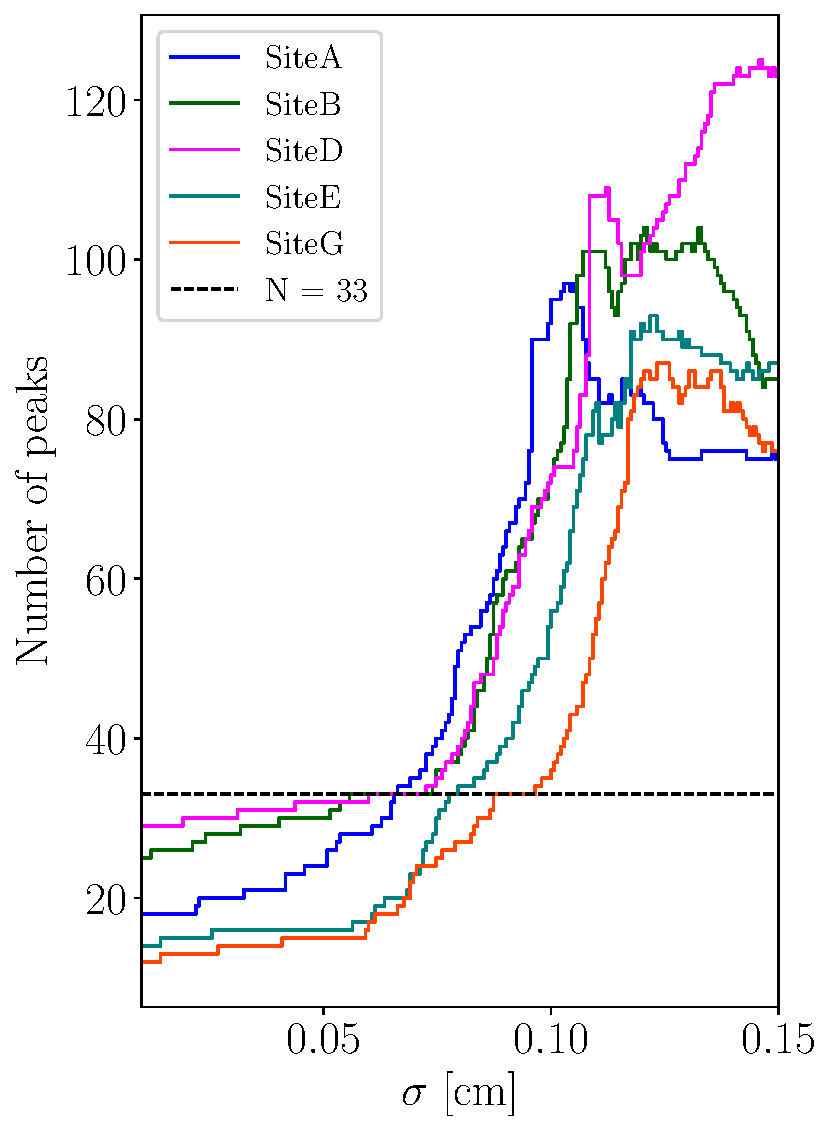
\includegraphics[width=\marginparwidth]{AllCores_NpeaksVDiffLen.pdf}
	\caption[$\sigma$ vs. N peaks]{\footnotesize Number of peaks estimated versus diffusion length, based on diffusion lengths in the interval [0.01; 0.15] m.}
	\label{Fig:AllCores_NpeaksVDiffLen}
\end{marginfigure}

%\begin{figure}
%	\begin{tikzpicture}[node distance=1.5cm, auto]
%		\node(start) [startstop] {START};
%		%----------------------------------------------------%
%		\node(in1) [io, left of=start, xshift=-2.5cm] {Depth series};
%		\node(empty1) [below of=in1, yshift=0.12cm] {};
%		\node(empty2) [below of=in1, xshift=-0.15cm] {};
%		%		\node(in1pro1) [process, below of=in1, yshift=-0.5cm] {Spline interpolation};
%		\node(in1pro2) [process, below of=in1, yshift=-2cm] {Spectral analysis};
%		\node(decSpec1) [decision, below of=in1pro2, scale = 0.8, align=center] {DCT ?\\(Interpolation)};
%		\node(decSpec2) [decision, left of=decSpec1, scale=0.8, xshift = -1.2cm, align=center] {FFT ?\\(Interpolation)};
%		\node(decSpec3) [decision, right of=decSpec1, scale=0.8, xshift = 0.8cm] {NDCT ?};
%		
%		\node(in1pro3) [process, below of=decSpec1] {Wiener filter};
%		
%		\draw[arrow] (in1) -- (start);
%		\draw[-] (start) |- (empty2);
%		\draw[arrow] (empty1) -- (in1pro2);
%		%		\draw[arrow] (in1pro1) -- (in1pro2);
%		\draw[arrow] (in1pro2) -- (decSpec1);
%		\draw[arrow] (in1pro2) -- (decSpec2);
%		\draw[arrow] (in1pro2) -- (decSpec3);
%		\draw[arrow] (decSpec1) -- (in1pro3);
%		\draw[arrow] (decSpec2) -- (in1pro3);
%		\draw[arrow] (decSpec3) -- (in1pro3);
%		%	\draw[arrow] (in1pro3) -- (in1pro4);
%		
%		%----------------------------------------------------%
%		
%		\node(in2) [io, right of=start, xshift=2.5cm] {Core specs};
%		\node(in2pro1) [process, below of=in2, yshift=-0.5cm] {Density profile};
%		\node(in2pro2) [process, below of=in2pro1] {Diffusion profile};
%		\node(in2pro3) [process, below of=in2pro2] {$\sigma_0$\textbf{ estimate}};
%		\node(decSigma1) [decision, below of=in2pro3, scale = 0.8] {$\sigma_0 = \sigma_{\text{const}}$?};
%		\node(decSigma2) [decision, right of=decSigma1, scale = 0.8, xshift=0.8cm] {$\sigma_0 = \sigma(z)$?};
%		\node(decSigma3) [decision, left of=decSigma1, scale = 0.8, xshift=-0.8cm] {$\sigma_0 = \sigma_{\text{input}}$?};
%		
%		
%		\draw[arrow] (in2) -- (start);
%		\draw[arrow] (start) |- (in2pro1);
%		\draw[arrow] (in2pro1) -- (in2pro2);
%		\draw[arrow] (in2pro2) -- (in2pro3);
%		\draw[arrow] (in2pro3) -- (decSigma1);
%		\draw[arrow] (in2pro3) -- (decSigma2);
%		\draw[arrow] (in2pro3) -- (decSigma3);
%		
%		%----------------------------------------------------%
%		\node(pro0) [process, below of=start, yshift=-6.5cm] {Frequency Filters};
%		\node(pro1) [process, below of=pro0,align=center] {\textbf{Deconvolution}\\(Uniform resampling)};
%		\node(stop) [startstop, below of=pro1] {\textbf{STOP}};
%		\node(out1) [io, right of=stop, align=center, xshift=2.2cm, text width=2.5cm] {\footnotesize{Back diffused depth series}};
%		\node(out2) [io, below of=out1, align=center] {\footnotesize{$\sigma_{\text{out}}$}};
%		\draw[arrow] (in1pro3) |- (pro0);
%		\draw[arrow] (decSigma1) |- (pro0);
%		\draw[arrow] (decSigma2) |- (pro0);
%		\draw[arrow] (decSigma3) |- (pro0);
%		\draw[arrow] (pro0) -- (pro1);
%		\draw[arrow] (pro1) -- (stop);
%		\draw[arrow] (stop) -- (out1);
%		\draw[arrow] (stop) |- (out2);
%		
%		%		\draw[arrow] (in2pro3) -| (pro0);
%		
%	\end{tikzpicture}
%	\caption[Flowchart of initialization method.]{\small Flowchart of initialization method for back diffusion of a depth series given a diffusion length estimate.}
%	\label{Fig:FlowchartBackDiffusion}
%\end{figure}

The algorithm does not contain an optimized version for determining the optimal varying $\sigma(z)$, and if $\sigma(z)$ is chosen, the algorithm searches linearly through $\sigma$ space, by moving the fitted $\sigma(z)$ through the diffusion length depth profile. This, along with the multiple deconvolutions with different Gaussian filters, makes this part of the algorithm very slow. This means that the further analysis does not focus on $\sigma(z)$, but future work could benefit from investigating this module further.

\subsection[Constrained Peak Detection]{Constrained Peak Detection}
\label{Subsec:Meth_PeakDetection_Constrained}
The main constraint when back diffusing these depth series is the number of years between the two volcanic events detected in the ice. The number of especially winters between the two events is fixed to $N_P=33$, as this number of winters is expected in the interval, even with a two month variation from the estimated event position. The counted number of summers can on the other hand vary a bit, due to the uncertainty on the exact time of deposition from the volcanic events, as discussed in Chapter \ref{Chap:Data}.\\
For better peak detection, a number of other constraints have been implemented. Since the data is a proxy for a continuous physical process, the temperature, it is reasonable to set up constraints representing some of the logical expectations for this type of signals. 

Firstly, restrictions may be demanded of the distance between peaks. The annual layer thickness, $\lambda_A$, may help with setting some limitations on the peak distances, as it is not likely for the average peak distance to be much smaller than $\lambda_A$. The peaks are expected to show the same annual cycle as the rest of the signal, representing summers. 

Secondly, for the prominence of the peaks, i.e. the amplitude of the signal at a depth, it is assumed that individual peaks may not have a prominence of less than a certain percentage of the standard deviation of the signal at the given depth. This makes certain that smaller peaks or troughs, maybe representing a warm period in a winter or a cold period in summer, are not counted as annual peaks or troughs. 
This is one way to constrain peak prominence, but a more efficient and accurate way is to consider the amplitude of the entire ice core signal. As it may be assumed that the amplitude and prominence at a given depth will be somewhat smaller than the prominence of the peaks at a shallower depth, due to the general diffusion in the firn. By analyzing the amplitude attenuation of the ice core, the average attenuation at a given depth could be used as a restriction for the peak prominence. This is something that would have been implemented, if time had allowed it.


Thirdly, a constraint on how the general pattern of the trough and peak detection must look is imposed. As the temperature variations represent the change from summer to winter, it is assumed that the general pattern must be able to detect a peak $P$, then a trough $T$, then a peak $P$, and so on, creating a pattern of $...PTPTPTP...$. Since the deposition time of volcanic material in the ice is assumed to be Gaussian, the pattern is not restricted to starting with either a peak or a trough, as this may vary when drawing a location from the distribution. Thus, the number of peaks is set at $N_P=33$ and the number of troughs is accepted with a variation, as long as the general pattern is intact.

Finally, the diffusion length estimate is kept at a positive value with an upper limit, that can be set manually, depending on the conditions of the site and the depth. 

The optimal parameter choices for the constraints are presented in Table \ref{Tab:ConstraintParams}.

\begin{table}[ht]
	\centering
	\begin{tabular}{lc}
		\toprule 	
		$N_P$ & 33\\[0.15cm]
		$N_T$ & $33\pm 1$\\[0.15cm]
		Peak(trough) prominence & 50 \% of $SD_{\text{signal}}$\\[0.15cm]
		Peak(trough) distance & 50 \% of $\lambda_A$\\[0.15cm]
		$[\sigma_{min}, \sigma_{max}]$ [cm] & [0, 15]\\[0.15cm]
		Pattern & $...PTPTPTPTP...$\\
		\bottomrule
	\end{tabular}
	\caption[Constraint parameters]{The general constraints used in the method to optimize the diffusion length estimate.}
	\label{Tab:ConstraintParams}
\end{table}

%\subsection[Corrections on $\sigma$][Corrections on $\sigma$]{Corrections on the Computed $\sigma$ estimate}
%\label{Subsec:Method_SigmaMethod_SigmaCorrections}
%As mentioned in Section \ref{Subsec:Ice_DiffusionAndDensification_Diffusion_TemperatureRecon}, the estimated diffusion length needs to be corrected for a number of different influences: the sampling diffusion, the ice diffusion at a given depth and the thinning function at a given drill site.
%
%This section will describe how each of these influences have been taken care of in the work.
%
%\subsubsection{Ice Diffusion, $\sigma_{\text{ice}}$}
%\label{Subsubsec:Method_SigmaMethod_SigmaCorrections_IceDiffusion}
%
%\subsubsection{Sampling Diffusion, $\sigma_{\text{dis}}$}
%\label{Subsubsec:Method_SigmaMethod_SigmaCorrections_SamplingDiffusion}
%
%\subsubsection{Thinning Function $S(z)$}
%\label{Subsubsec:Method_SigmaMethod_SigmaCorrections_ThinningFct}




%\subsection[$1^{\text{st}}\sigma$ Estimate][$1^{\text{st}}\sigma$ Estimate]{$1^{\text{st}}$ Diffusion Length Estimate}
%\label{Subsec:Method_SigmaMethod_1stEstimate}

%\subsection[Optimal $\sigma$ Estimate][Optimal $\sigma$ Estimate]{Optimal Diffusion Length Estimate}
%\label{Subsec:Method_SigmaMethod_OptEstimate} 


\section[Testing and Stability][Testing and Stability]{Method Testing and Stability}
\label{Sec:Method_TestStab}

Throughout this section a number of different tests of the algorithm will be presented. The tests are performed to examine the stability of the method, the accuracy of the Laki and Tambora positions and how the choice of parameters (interpolation, spectral transform type) changes the resulting diffusion length estimate. 

\subsection[Constraints or No Constraints]{No constraints versus constraints}
\label{Subsec:Method_TestStab_ConstNoConst}
Figure \ref{fig:SiteB_ConstVNoConst} shows the depth series between Laki and Tambora events of the ice core drilled at Site B, back diffused through the algorithm described in the above. The difference between the blue and the green back diffused signals is that the blue is back diffused using the above presented constraints, and the green signal is back diffused with only the constraint $N_P=33$. It is clear that the imposed constraints, especially the ones concerning peak distance and prominence, influence the final result of the optimal diffusion length. Particularly, the algorithm containing more constraints clearly leaves out some 'shoulders' before an actual peak in the final count, see Figure \ref{fig:SiteB_ConstVNoConst} at a depth of 77.5 m. These shoulders could be actual peaks but with the imposed constraints, they are omitted. This is something that could be further developed and examined. The appearance of these 'shoulders' could be peaks, but it is also likely that they are remnants of some noise effect that is not quite filtered in the frequency filter construction. If that is the case, then it is a positive thing that the algorithm filters them out.

\begin{figure}[!htb]
	\centering
	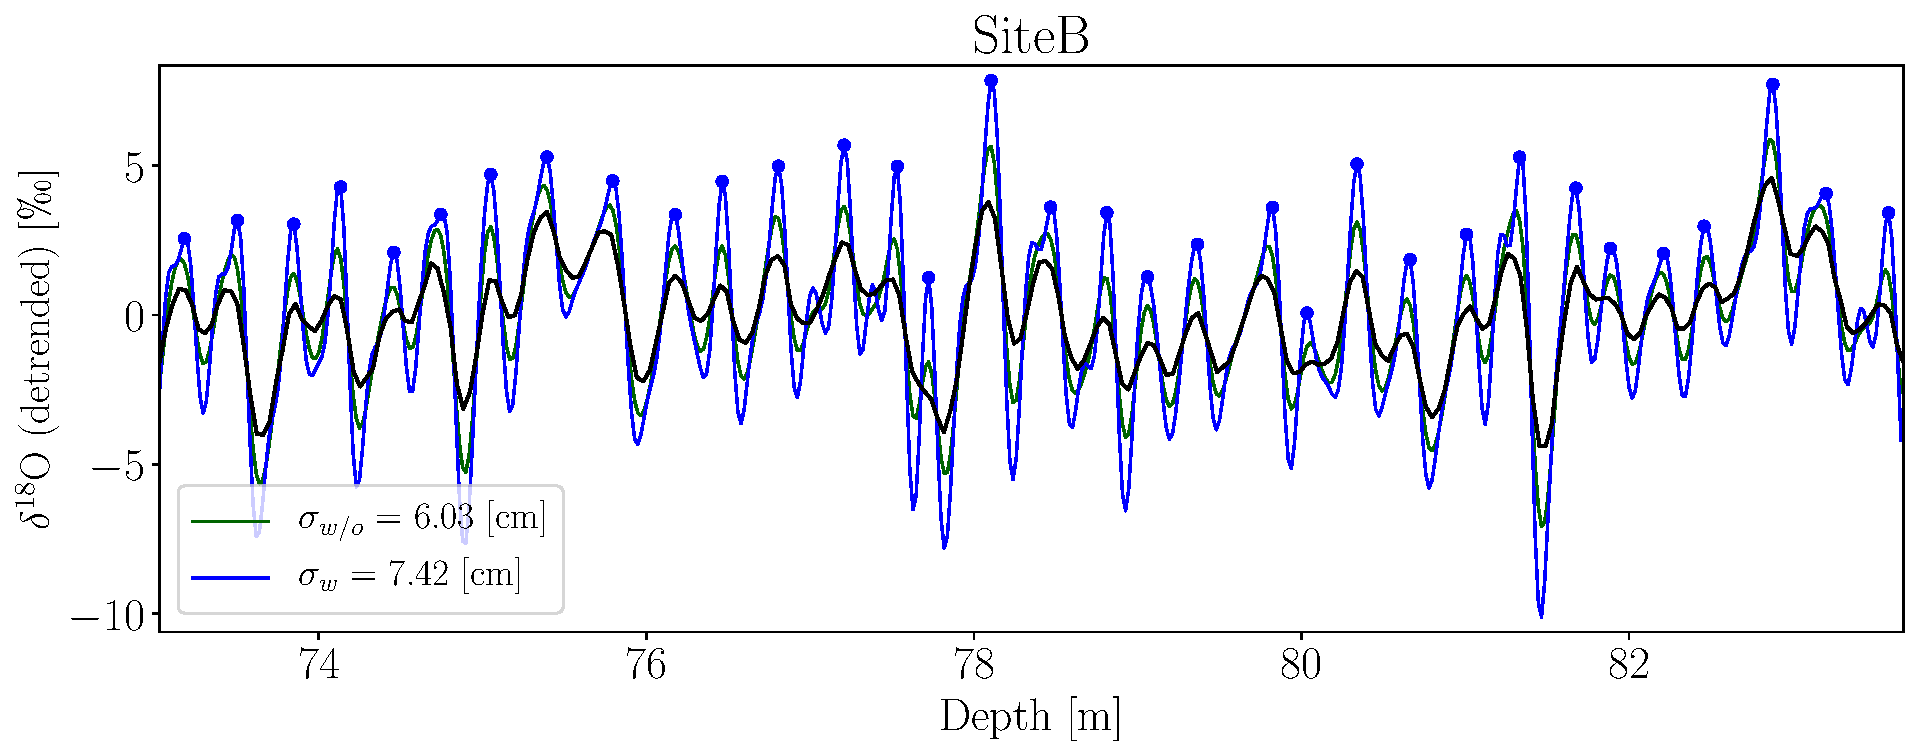
\includegraphics[width=\textwidth]{SiteB_ConstVNoConst.pdf}
	\caption[Site B constrained vs. unconstrained]{\small Example of how the imposed constraints affect the final diffusion length estimate for the Laki to Tambora depth section of the core drilled at Site B. The black line shows the data, the green the back diffused data using a method with less constraints, and the blue line shows the back diffused data when using the imposed constraints. The blue dots represent the peaks counted in the constrained method.}
	\label{fig:SiteB_ConstVNoConst}
\end{figure}


\subsection[Effects of Interpolations]{Effects of Interpolations}
\label{Subsec:METH_Interpolation}
The choice of interpolation, before and after deconvolution, does affect the final result by introducing some effects not inherent in the originally measured signal. Therefore it is important to examine exactly how these interpolations influence the final $\sigma$ estimate. Here that is examined by running the algorithm with different resampling sizes. 

\subsubsection[Interpolation 1]{Interpolation of Data Before Deconvolution}
\label{Subsubsec:METH_Interpolation_BFdecon}
\begin{figure}[!htb]
	\centering
	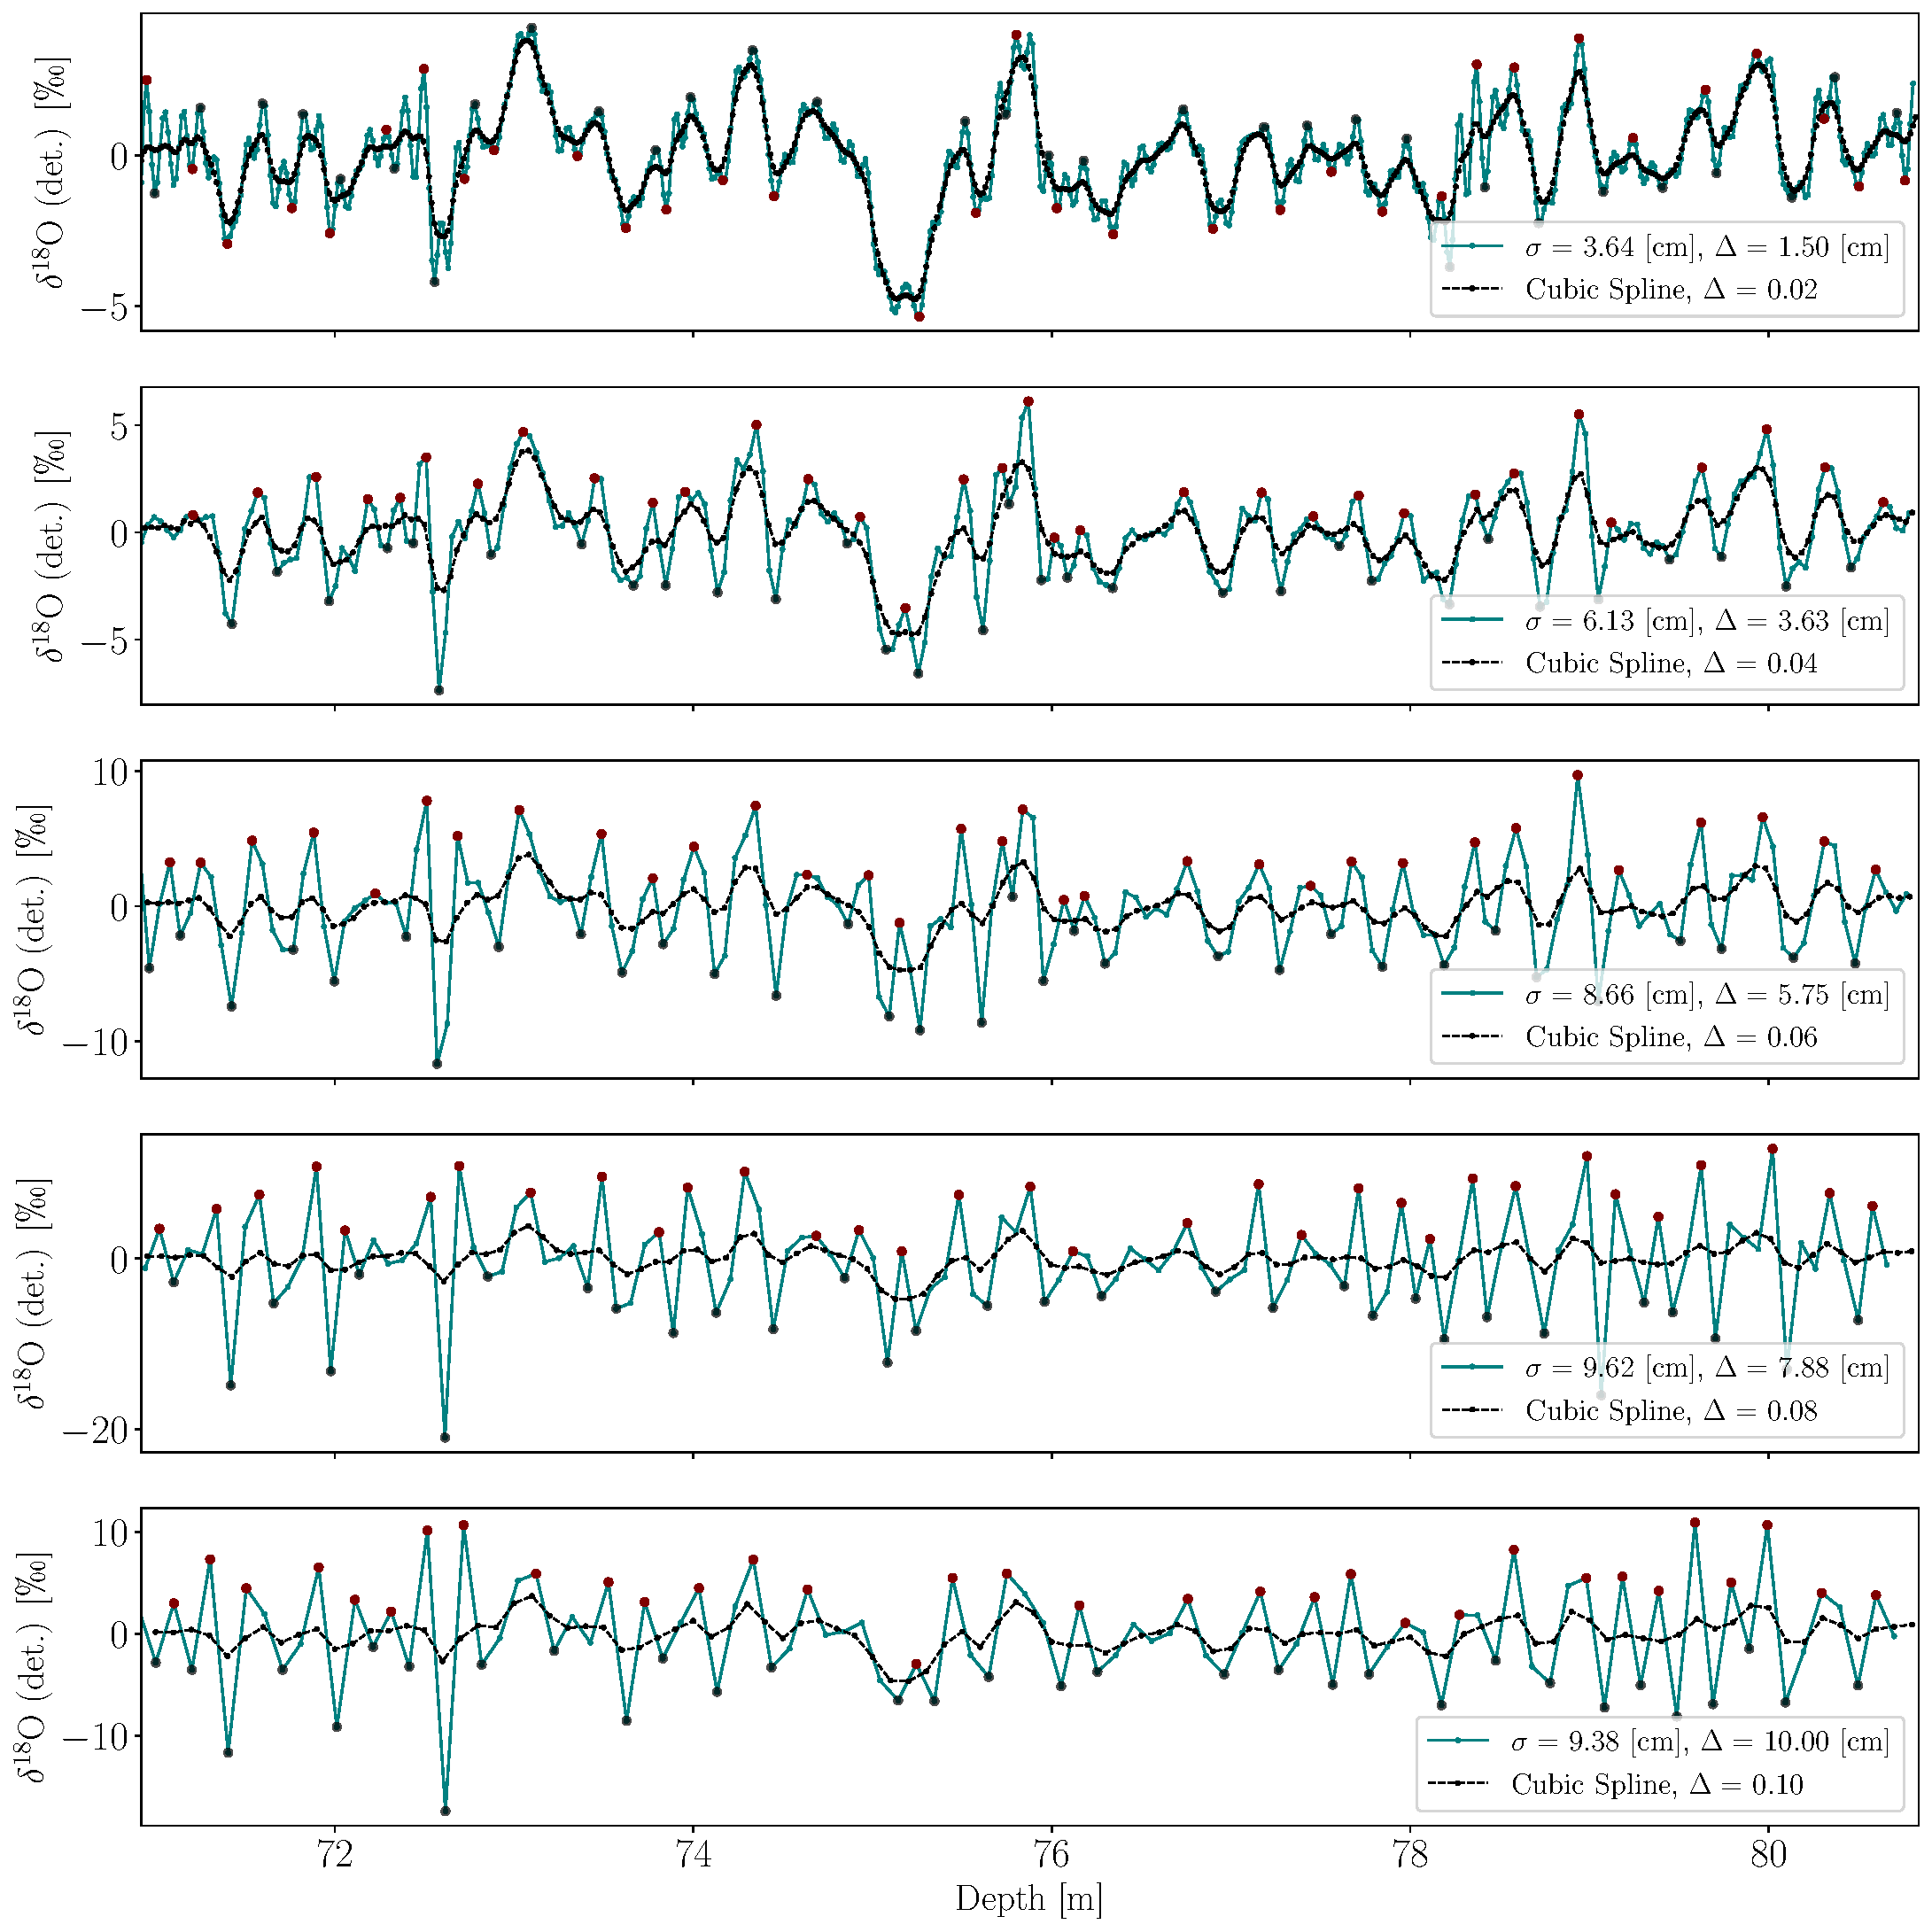
\includegraphics[width=\textwidth]{SiteA_InterpBF_SpecificResamplings.pdf}
	\caption[BD data, Site A, resamplings before deconvolution]{\small Site A, illustration of the effect of five different cubic spline resamplings before deconvolution. Original sample sizes lie in the interval [3.80; 4.00] [cm]. Resampling at smaller sample sizes show a tendency to restore some signal frequencies that are not necessarily inherent to the original signal. The resample should thus not be chosen too small as this would introduce some false signal into the results.}
	\label{Fig:COMPMETH_SiteA_interpBF_SpecificSamplings}
\end{figure}

The first interpolation is needed if the fast spectral transforms FFT or FCT are used, as one of the conditions of the algorithms is that the data are evenly spaced. At first, this was implemented in the analysis, but this had the risk of excluding some information that might lie in the unevenly sampled data. Later, the method was abandoned in favor of implementing a nonuniform spectral transform (NUFT or NDCT), which is slower than the FFT and FCT, but carries all information from the unevenly sampled signal into the spectral domain. Luckily, this nonuniform transform needs only be carried out once, as the inverse transform, i.e. resampling in time domain, can be done uniformly without loss of information and any future spectral transforms can then be performed through FFT or FCT.

Even though the first interpolation method was later abandoned, some analysis was carried out with it to examine the effect of the size of the resampled, interpolated data on the final diffusion length estimate. Examples of a resampled signal can be seen in Figure \ref{Fig:COMPMETH_SiteA_DataSplineInterp} and Figure \ref{Fig:COMPMETH_SiteA_MultiSplineInterp}. Figure \ref{Fig:COMPMETH_SiteA_MultiSplineInterp} shows how sample resolution affects information from the signal. The higher sampling resolution, the more information is retained. But higher sampling resolution also means more data to be analyzed, which might slow down any analysis algorithms developed. This might create some headache if an entire ice core length of a couple thousand meters should be examined, but for this study only af few meters are of interest, and thus it should not create delays in the computation time.

To examine the effect of the resampling resolution on the final diffusion length estimate when conducting a spline interpolation before carrying out the back-diffusion, the full diffusion length analysis has been performed with 100 new interpolation resampling sizes in the range $[\Delta_z^{\text{min}};\Delta_z^{\text{max}}]$. This gives an idea of the stability of the method considering both sample size of the raw data and resampling by interpolation. The minimum and maximum interpolation samplings are presented in Table \ref{tab:InterpSamples} and an illustration of the test results can be seen in Figure \ref{Fig:COMPMETH_SamplingVsDiffLen_interpBF}. 

Figure \ref{Fig:COMPMETH_SamplingVsDiffLen_interpBF} shows that if the sampling size of the interpolation is decreased, it becomes difficult for the algorithm to determine a diffusion length that fulfills the constraints. This is due to the spectral transforms and back diffusion method being sensitive to small variations that the spline interpolation introduces to the signal, as can be seen in the first panel in Figure \ref{Fig:COMPMETH_SiteA_interpBF_SpecificSamplings}. Furthermore, Figure \ref{Fig:COMPMETH_SamplingVsDiffLen_interpBF} shows a less stable diffusion length estimate as the resampling size increases, and a general tendency to result in higher diffusion lengths as many features become washed out in the signal and need more enhancement by cranking up the diffusion length estimate, see final panel in Figure \ref{Fig:COMPMETH_SiteA_interpBF_SpecificSamplings}. The interpolation before deconvolution is only necessary for running the method with the spectral transforms that are based on uniform sampling, i.e. the FFT and the DCT. For these two methods a choice of interpolation size can be made, but the general setting in the algorithm is to resample at the smallest sampling size found in the depth interval, $\Delta_z^{\text{min}}$.
\marginnote{%
	\footnotesize
	\centering
	\begin{tabular}{lccc}
		\toprule
		\textbf{Site} & $\Delta_z^{\text{min}}$& $\Delta_z^{\text{max}}$ & $\Delta_z^{\text{OG}}$\\
		& [cm] & [cm] & [cm] \\
		\midrule
		A & 1.0 & 10.6 & 3.8-4.0\\
		B & 1.0 & 11.7 & 3.8-4.0\\
		D & 1.0 & 12.0 & 3.7-3.9\\
		E & 1.0 & 11.4 & 4.1-4.4\\
		G & 1.0 & 10.3 & 4.0-4.2\\
		\bottomrule
	\end{tabular}
	\captionof{table}[Tested sample resolutions for resampling before back-diffusion]{\footnotesize Minimal and maximal new sample resolution used for testing interpolation before back-diffusion. Each test is run with 100 different new sample resolutions between $\Delta_z^{\text{min}}$ and $\Delta_z^{\text{max}}$.}
	\label{tab:InterpSamples}
}[0.5cm]%


\begin{figure}[!htb]
	\centering
	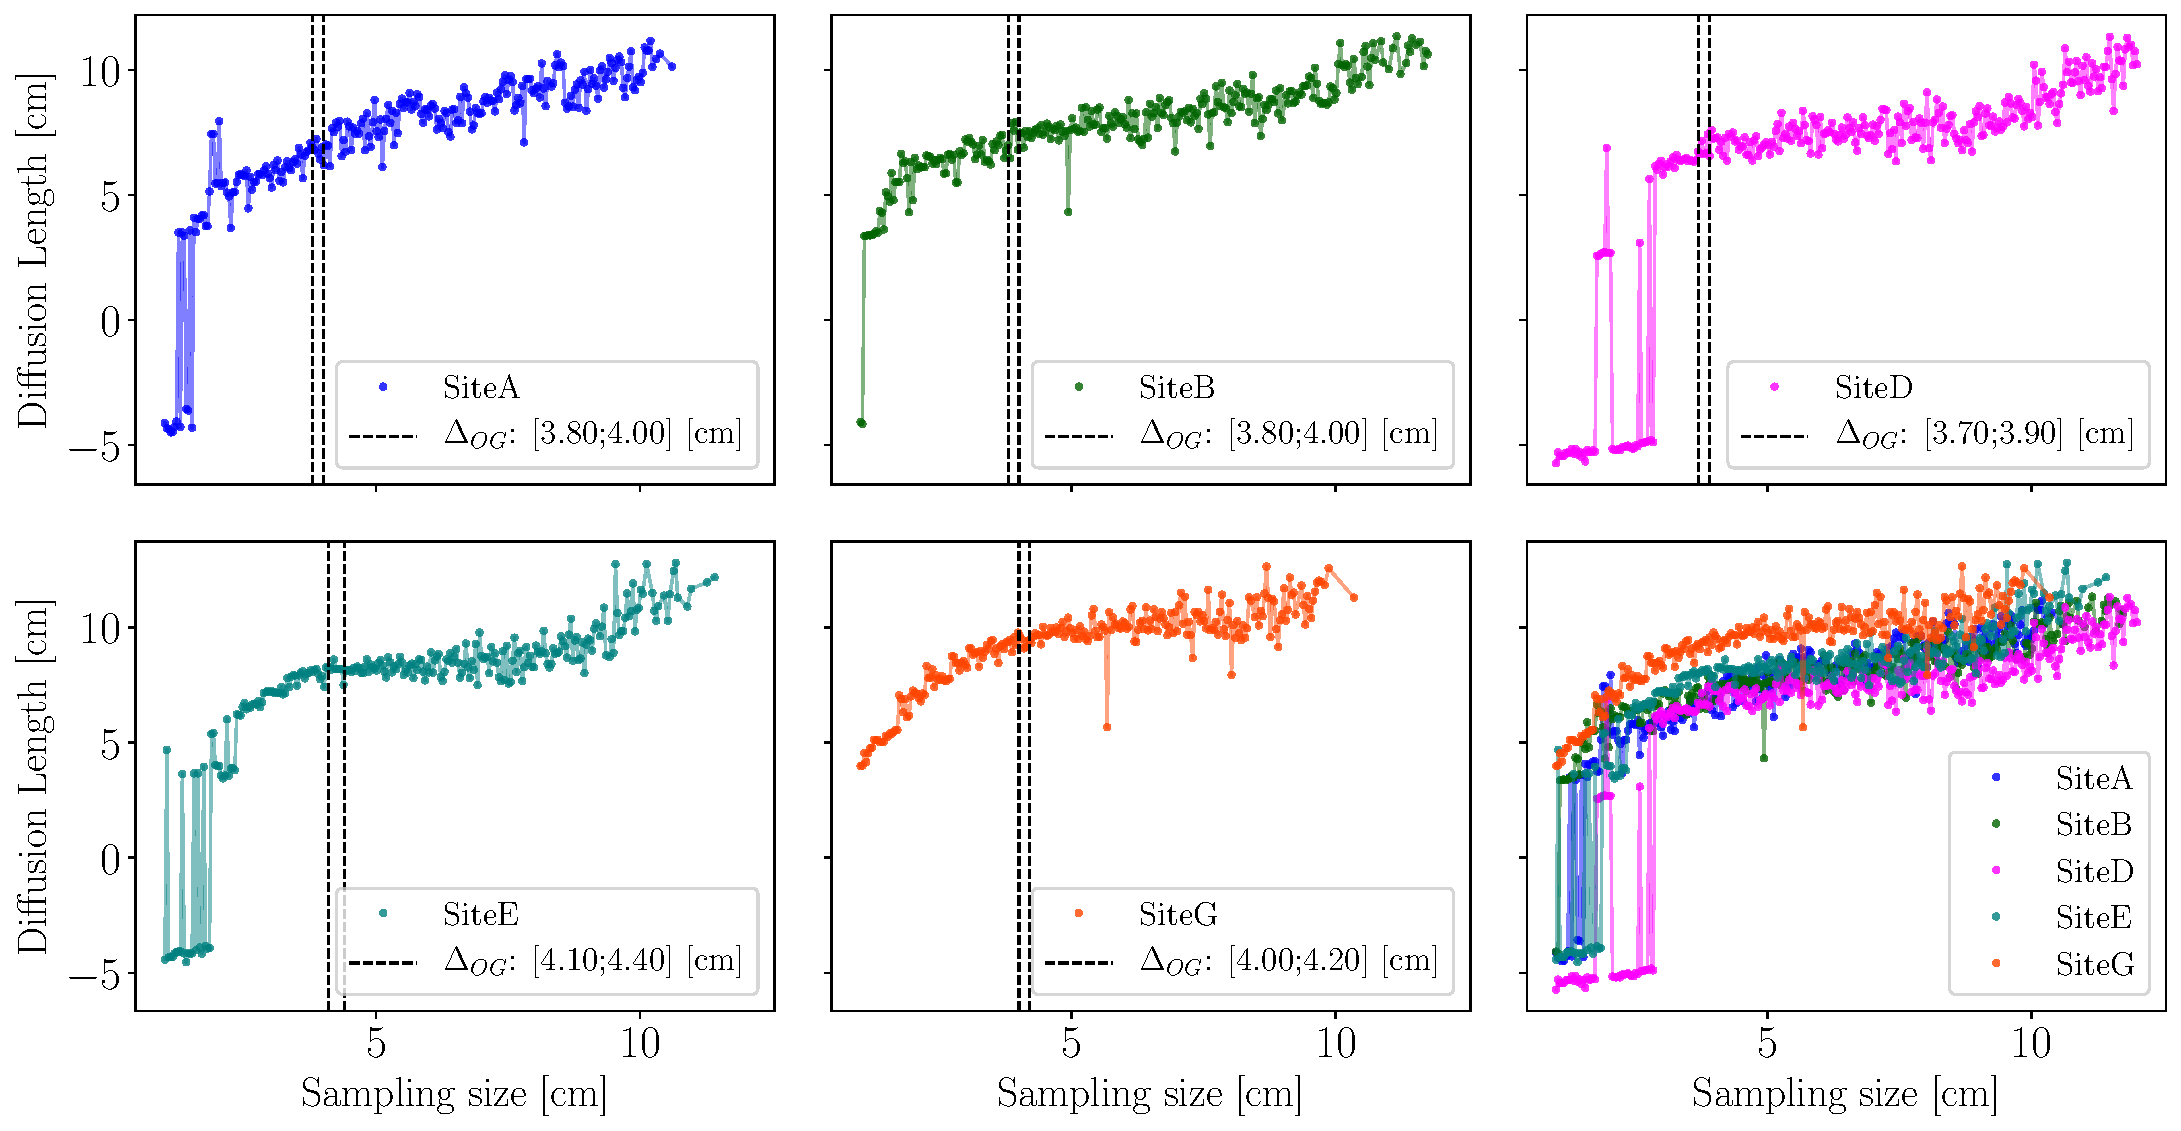
\includegraphics[width=\textwidth]{AllCores_DiffLenVdelta_InterpBF_const.pdf}
	\caption[$\sigma$ vs. resampling size before deconvolution]{\small Diffusion length estimates versus resamples through cubic spline interpolation before deconvolution for Alphabet cores from sites A, B, D, E and G.}
	\label{Fig:COMPMETH_SamplingVsDiffLen_interpBF}
\end{figure}



\subsubsection[Interpolation 2]{Interpolation of Data After Deconvolution}
\label{Subsubsec:METH_Interpolation_AFdecon}
\begin{figure}[!htb]
	\centering
	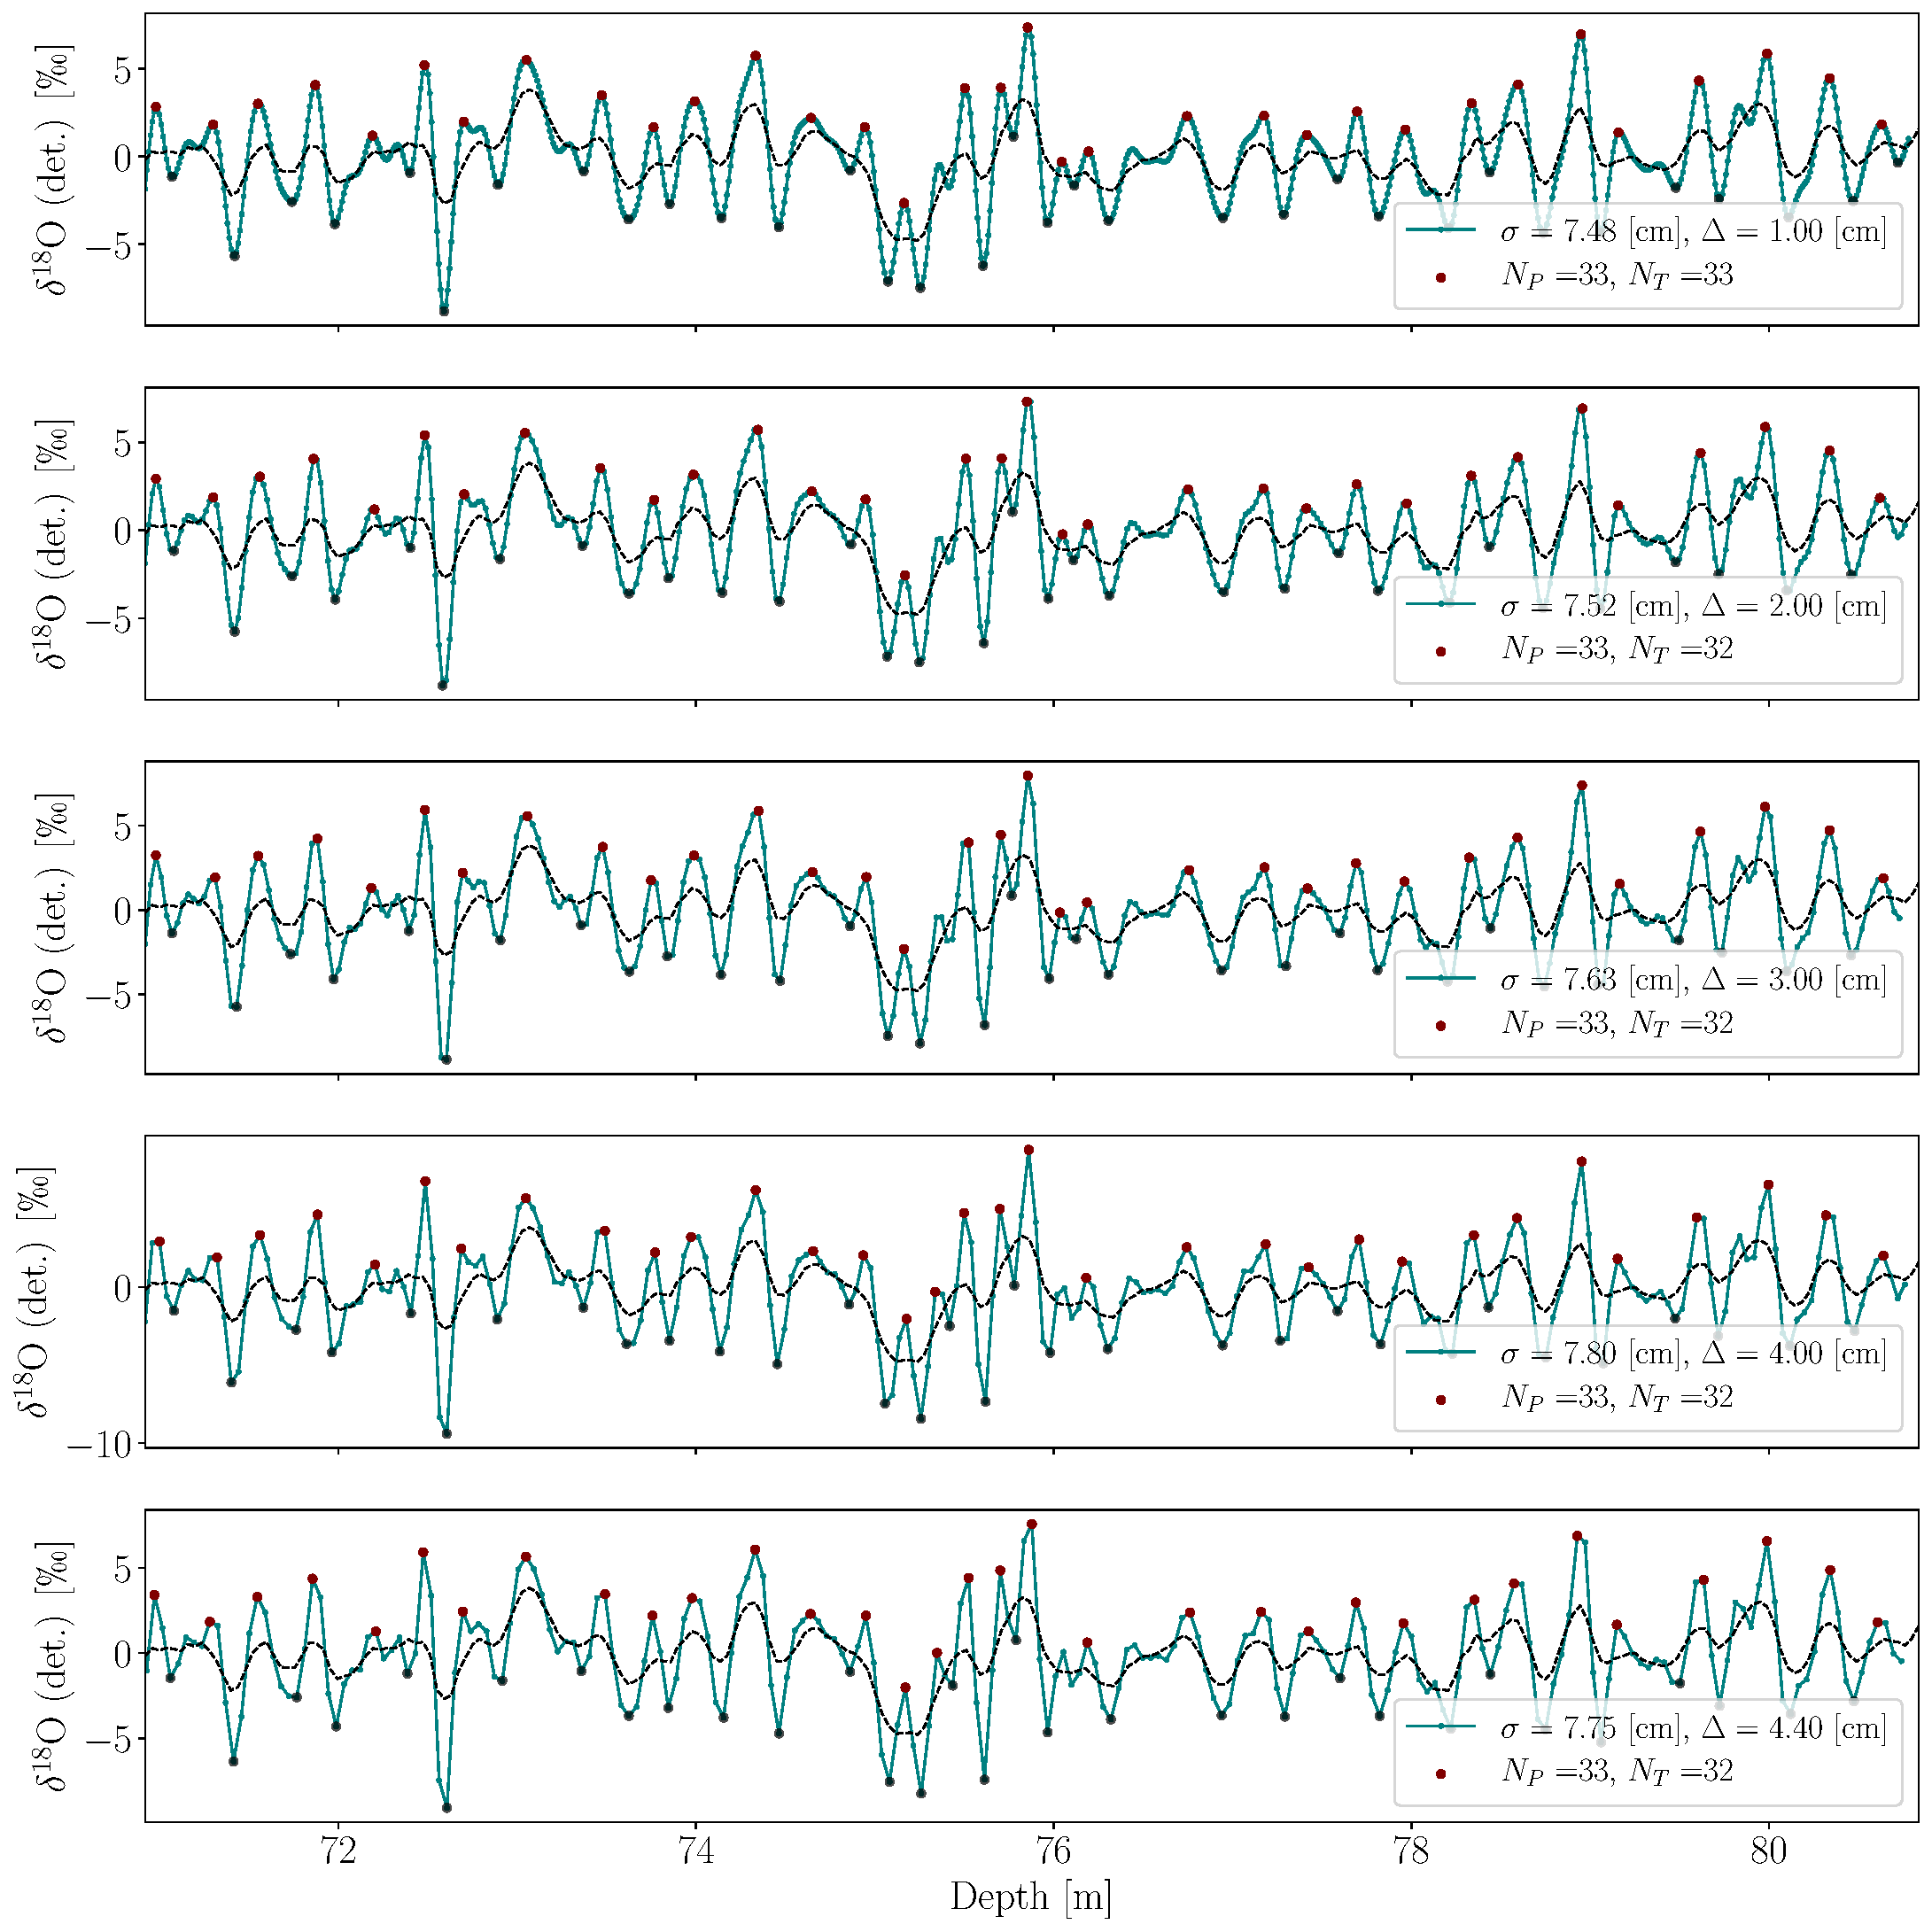
\includegraphics[width=\textwidth]{SiteA_InterpAF_SpecificResampling_BD.pdf}
	\caption[BD data, Site A, resamplings after deconvolution]{\small Site A, effect of cubic spline interpolation after signal has been deconvoluted. The interpolation is introduced to make peak detection more stable.}
	\label{Fig:COMPMETH_SiteA_InterpAF_4samplings}
\end{figure}

The second interpolation is carried out after deconvoluting and back-diffusing the signal, but before detecting peaks. Splines are especially effective when trying to find features like peaks in data whose underlying signal is continuous, smooth and differentiable, but the sampling is discrete and thus the data are discrete and non-smooth. The isotopic signal under examination here is assumed to be truly smooth and continuous throughout the core - unless any gaps are present. Thus the cubic spline interpolation is a good tool for estimating a higher resolution version of the final back-diffused data series to use for peak detection. This makes the detection of peaks and troughs more precise, as there might not be a discrete data point exactly at the top of a peak, but the spline interpolation then estimates where the most likely top of the peak must be, on the basis of the existing data. Examples of three different interpolation samplings are presented in Figure \ref{Fig:COMPMETH_SiteA_InterpAF_4samplings}. The effect of resampling after deconvolution on the final diffusion length estimate is illustrated in Figure \ref{Fig:COMPMETH_SiteA_InterpAF_4samplings}. 

As the actual isotopic signal is continuous and the discretization is introduced by different measurement samplings, it is assumed that the spline interpolation after deconvolution results in a more likely peak detection, when decreasing the numerical resampling size. In Figure \ref{Fig:COMPMETH_AllCores_SamplingVsDiffLen} the diffusion length estimate versus the resampling size after deconvolution can be seen, and the data show a convergence towards a fixed diffusion length as sampling size is decreased, and a much noisier diffusion length estimates as sampling size is increased. Furthermore, at certain larger sampling sizes the sought after pattern of peaks and troughs is not even reached. This resampling is carried out both for the FFT, DCT and NDCT spectral analysis methods, as the inverse NDCT can be resampled uniformly without any loss of information. Based on these observations, a resample size of $\Delta_z^{\text{min}}/2$ is chosen for interpolation after back diffusion and before peak detection. It is a compromise between choosing an interpolation that results in a higher resolution, but doing so without slowing down the algorithm too much. 



\begin{figure}[!htb]
	\centering
	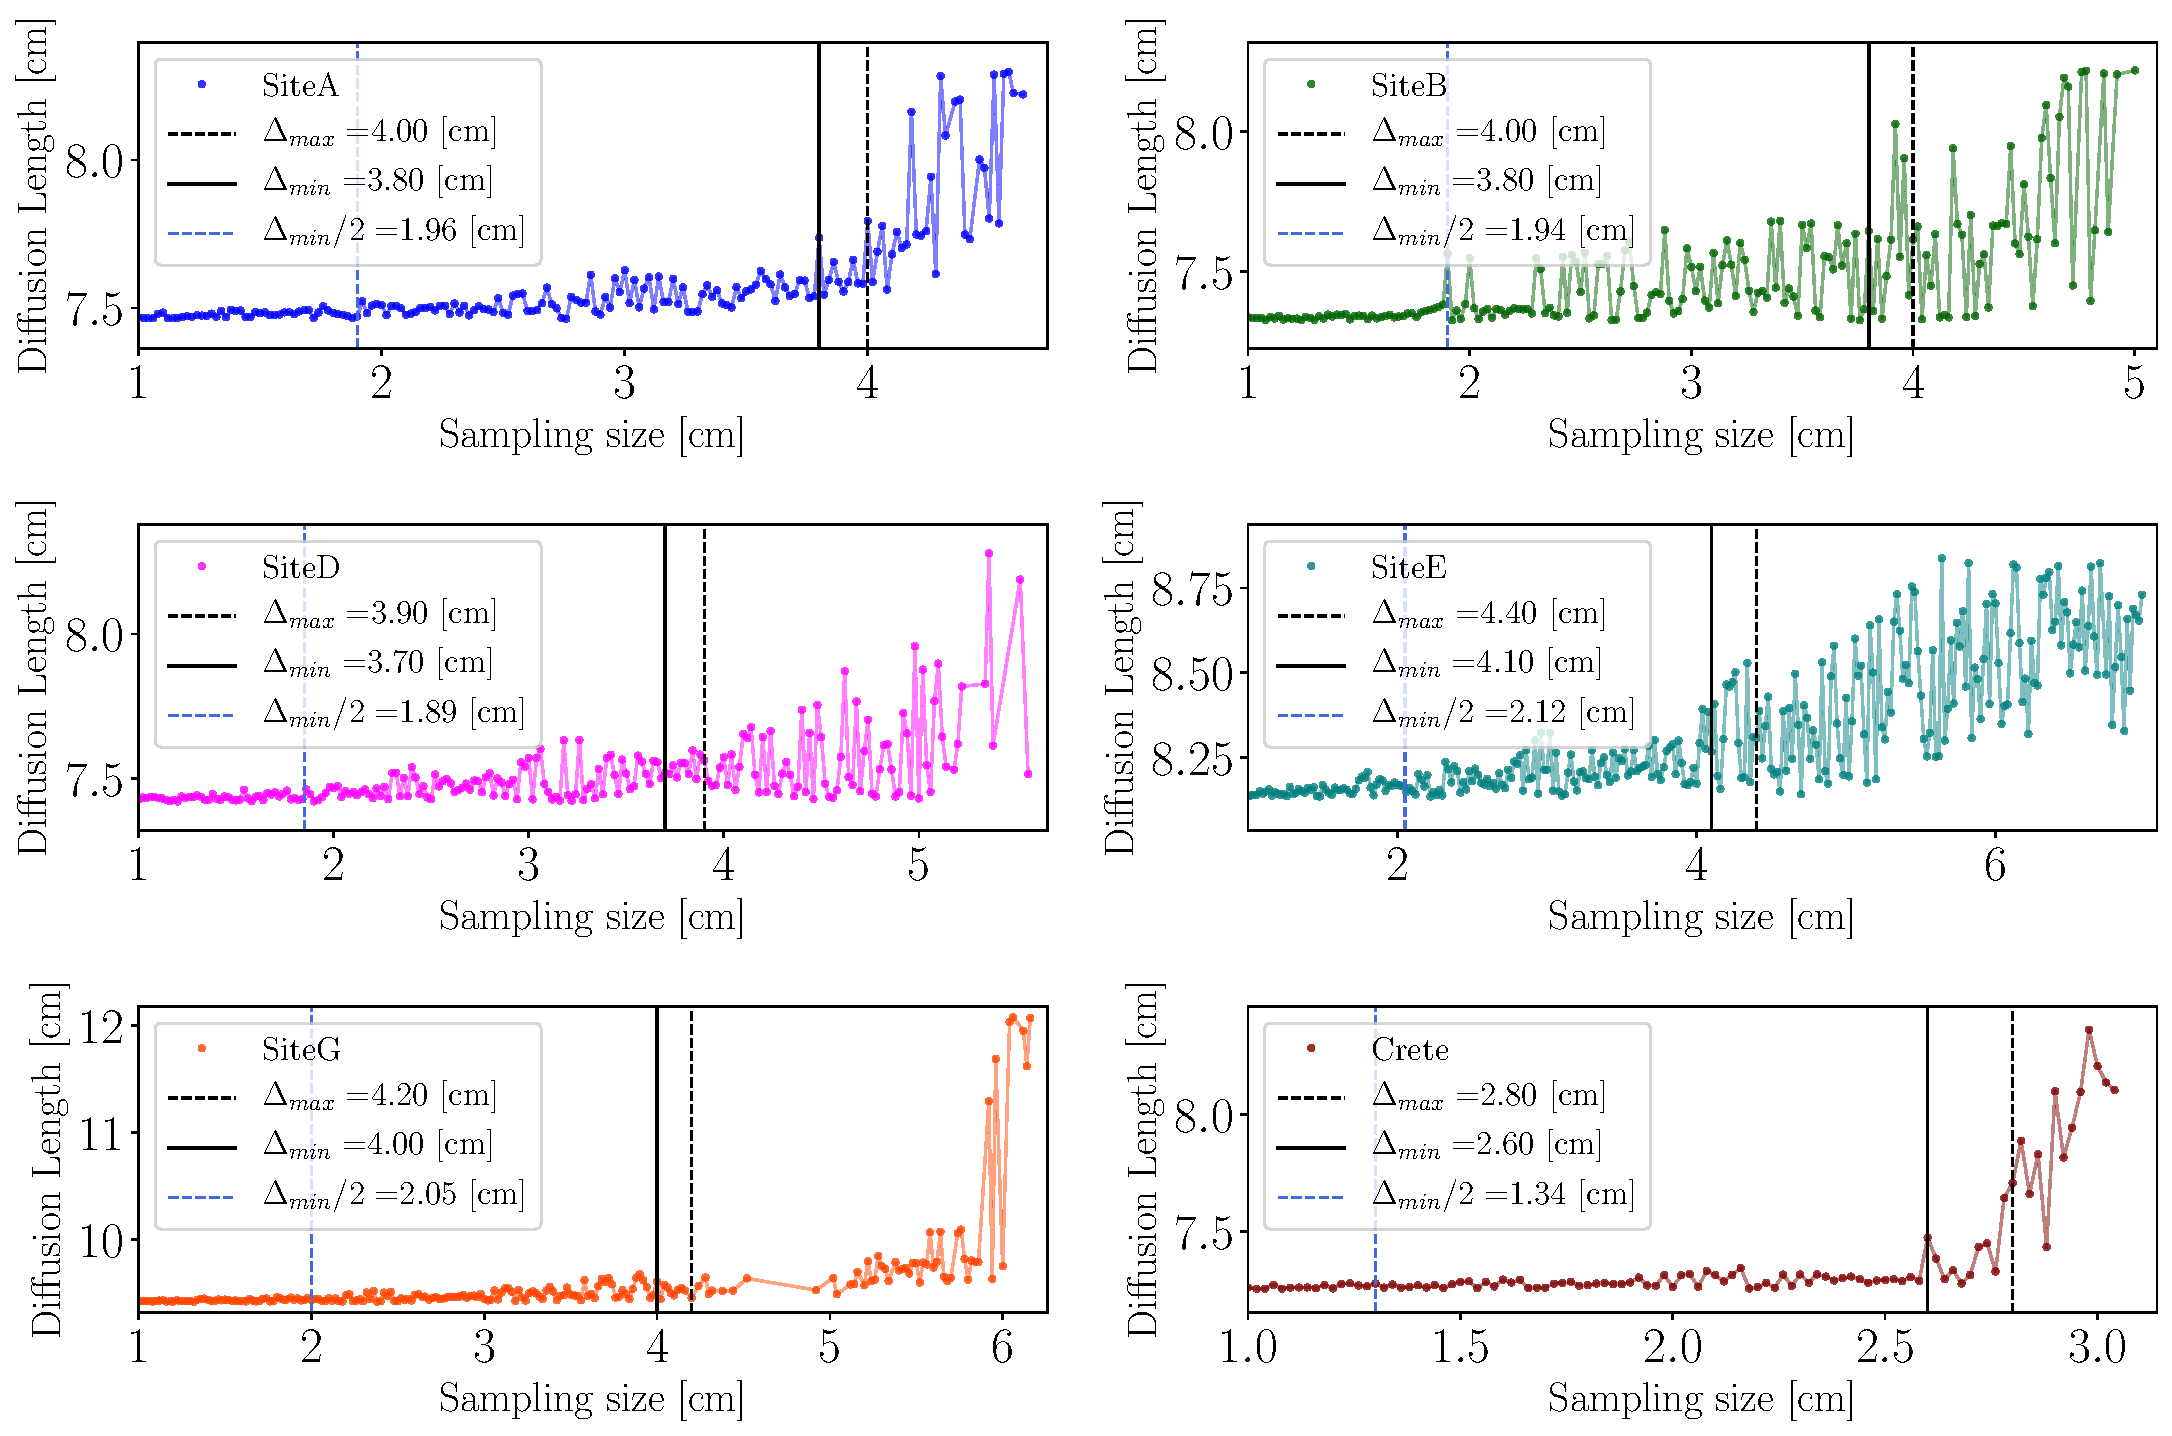
\includegraphics[width=\textwidth]{AllCores_InterpAF_deltaVSdiffLen_BD.pdf}
	\caption[$\sigma$ vs. resampling size after deconvolution]{\small Final diffusion length estimate, given new resample by cubic spline interpolation after deconvolution for Alphabet cores from sites A, B, D, E and G. The original sample size interval is illustrated as black vertical lines.}
	\label{Fig:COMPMETH_AllCores_SamplingVsDiffLen}\textit{}
\end{figure}


\subsection[Spectral Transforms]{Spectral Transform's Effect on Diffusion Length}
\label{Subsec:Method_TestStab_SpecTrans}
The different ways of performing spectral transformation also influence the final $\sigma$ estimate, not only due to the transformation itself, but for FFT and DCT, the methods demand an interpolation, which in itself influences the results. 

\begin{figure}[!htb]
	\centering
	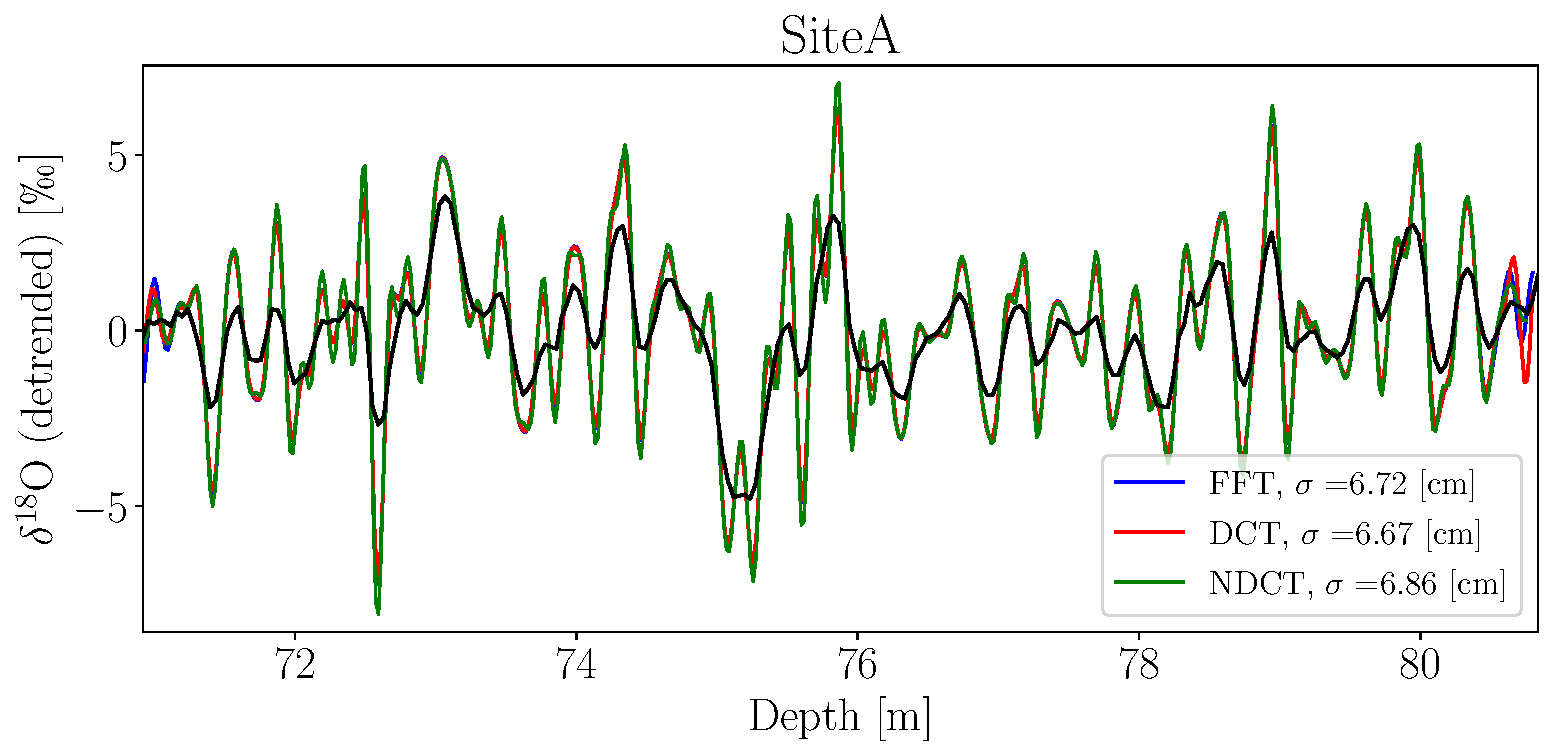
\includegraphics[width=0.8\textwidth]{SiteA_SpecTrans_VisInspection.pdf}
	\caption[Spectral transform's effect on $\sigma$]{\small A visual example of the differences in final back diffused data when using different spectral transforms. }
	\label{Fig:SiteA_SpecTrans_VisInspection}
\end{figure}

Figure \ref{Fig:SiteA_SpecTrans_VisInspection} shows an example of the qualitative differences between using FFT, DCT or NDCT for spectral analysis. The most obvious visual difference between the transforms is in the end sections of the interval. This might be due to some specific boundary conditions imposed on the fast Fourier and Cosine transforms. Furthermore, by careful visual inspection, it can be seen that the NDCT seems to cater to some effects of the nonuniform samplings, that the FFT and DCT do not.

There are no significant differences between the three spectral transforms, but there is some small variations. What might also be taken into consideration is, that this method might be run a large number of times - as is the case later on in this thesis - for example to estimate accuracy of the method, and one might therefore want to choose the method that gives the fastest results. Thus, the speed of the different transforms has been tested, as can be seen in Figure \ref{fig:SiteA_SpecTrans_Speed}, with 200 separate runs where the Laki and Tambora positions have been drawn from a distribution with a standard deviation of 2 months from the estimated location. Not surprisingly, the NDCT is much slower than the DCT and the FFT, and it might prove efficient to choose either DCT or FFT if the algorithm has to run many times. For the case of this thesis, the final results have been made with the NDCT, so as not to miss any of the effects that might come from unevenly sampled data.

\begin{figure}[!htb]
	\centering
	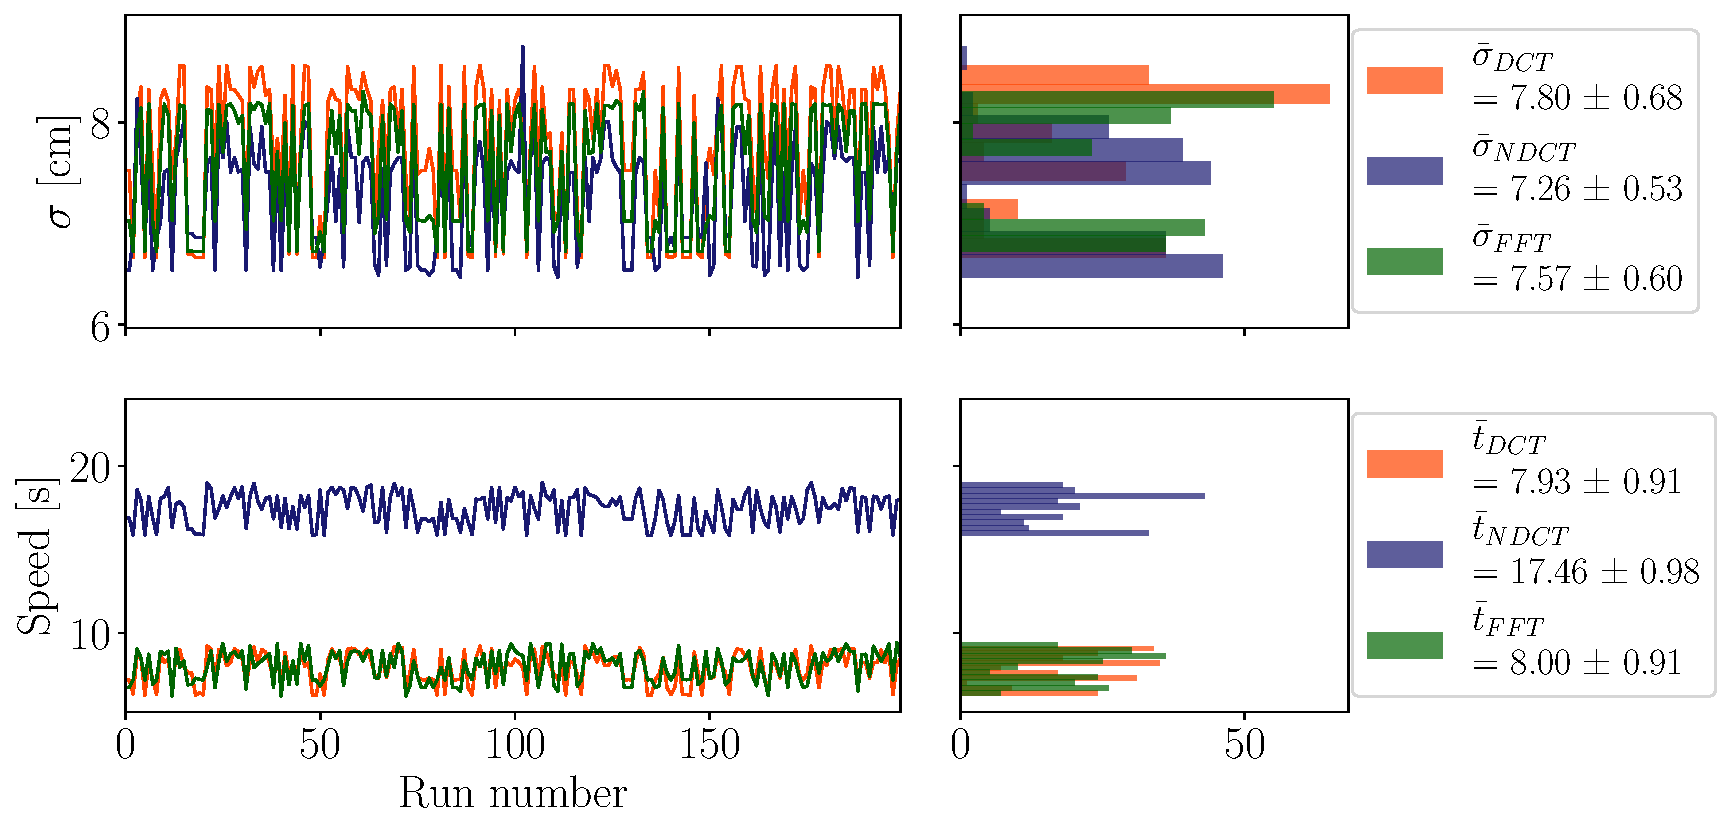
\includegraphics[width=0.95\textwidth]{SiteA_SpecTrans_Speed.pdf}
	\caption[Speed and $\sigma$ estimates, spectral transforms]{\small Diffusion length estimates along with speed of algorithm given the three different spectral transforms examined in this work. The volcanic event depths have been drawn from a Gaussian distribution with a width corresponding to $\sim$ 1 month around the estimated mean depth of the event.}
	\label{fig:SiteA_SpecTrans_Speed}
\end{figure}




\subsection[LT locations]{Laki and Tambora as Gaussian Distributions}
\label{Subsec:Method_TestStab_LTlocations}
As mentioned previously, the Laki and Tambora event depth locations are not exact. Thus to accommodate error in this positioning, the algorithm has been tested with Laki and Tambora locations drawn from Gaussian distributions. This was examined in four ways:

\begin{itemize}
	\item Variation in both Laki and Tambora position, corresponding to the entire events.
	\item Variation in only the Tambora position while keeping a fixed section length, corresponding to the mean value $\bar{d}_{L}-\bar{d}_{T}$.
	\item Variation in only the Laki position while keeping a fixed section length, corresponding to the mean value $\bar{d}_{L}-\bar{d}_{T}$.
	\item Variation corresponding to a Gaussian distribution with a standard deviation of a depth that resembles to months in time.
	
\end{itemize}

The first variation of both Laki and Tambora can be seen in Figure \ref{fig:SiteA_Vary_LandT}. The method has been run 500 times with new locations drawn for each run, and the same constraints imposed each time. This results in an estimate of the diffusion length for Site A between Laki and Tambora of $\sigma=7.32\pm 0.67$ [cm]. But considering the lengths of the volcanic events, as seen in the ECM data, one might question this result. Due to more or less time incorporated as the depth section is widened or narrowed, some of the constraints might not be very well chosen any more. It might be that a larger depth interval could gain an extra peak or trough, so that the constraint should be $N_P=34$ instead of $N_P =33$. This is some work that could be continued on the algorithm, ensuring that the extra interval length increase or decrease loosens the count constraint.

%\subsubsection[Vary L and T]{Varying both Laki and Tambora Position}
%\label{Subsubsec:Method_TestStab_LTlocations_LandT}

\begin{figure}[!htb]
	\centering
	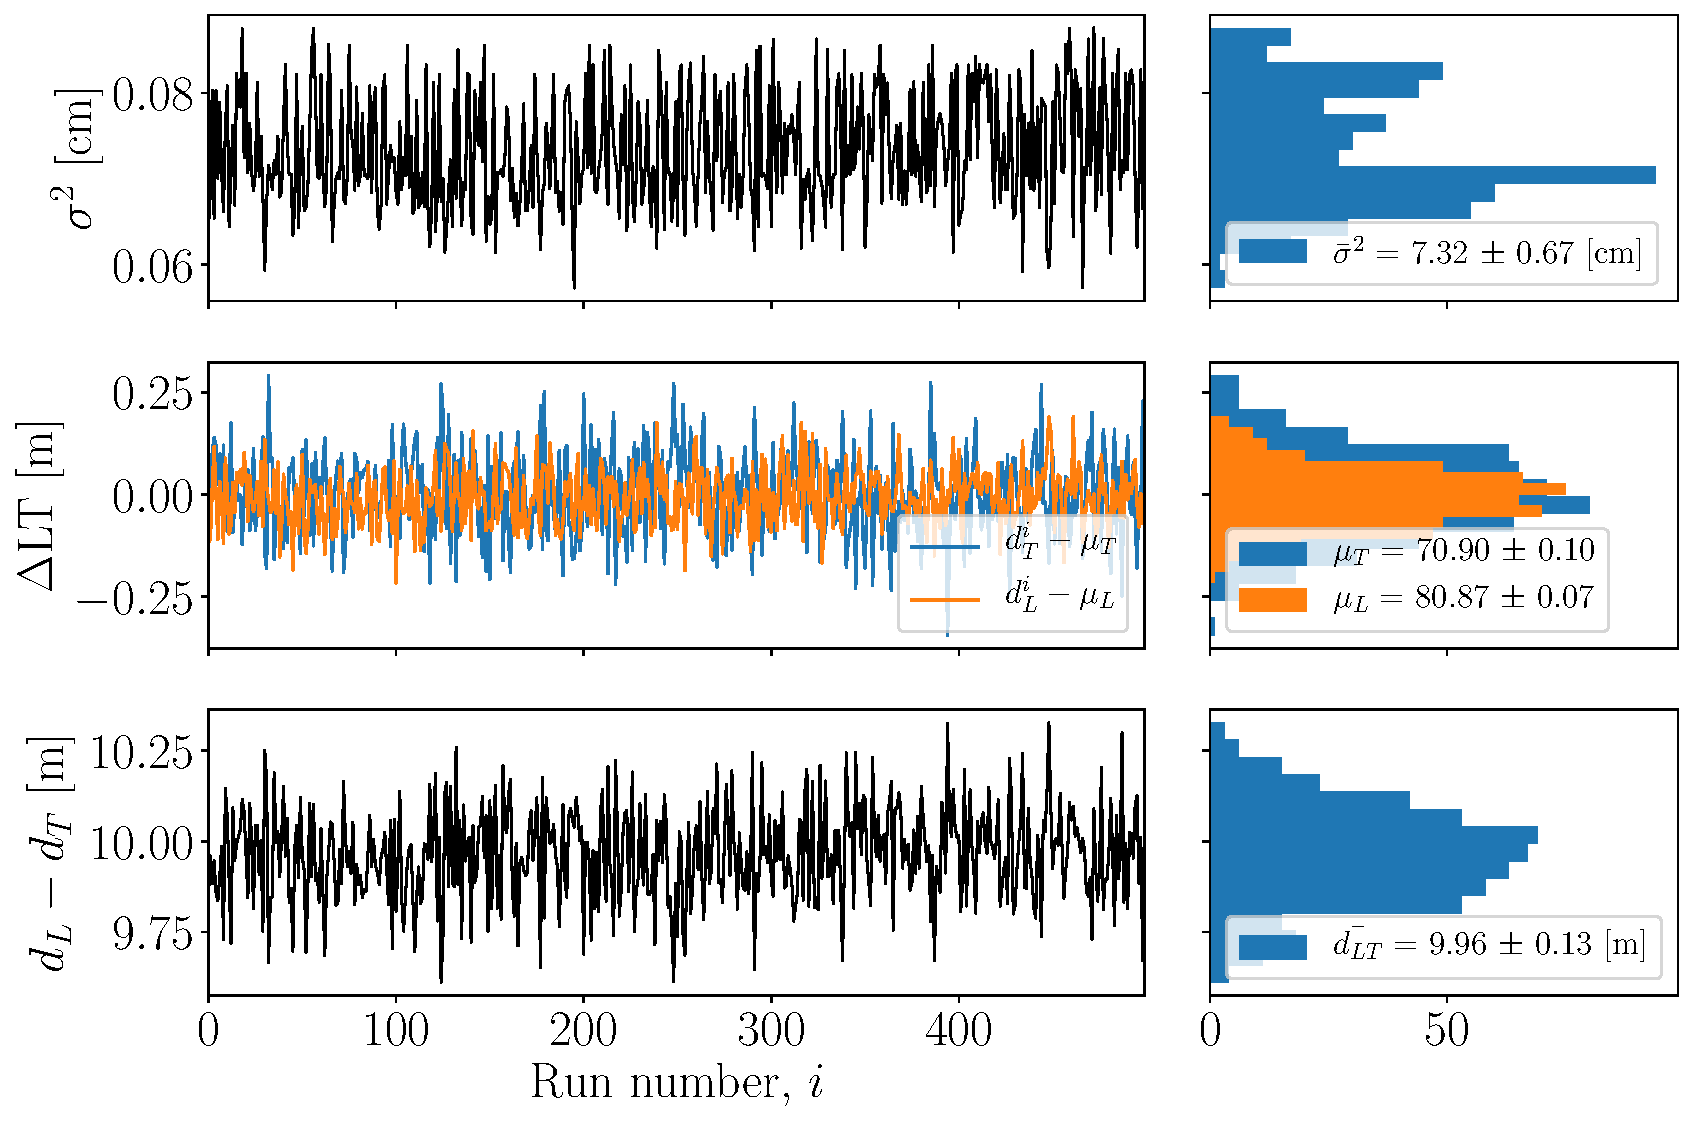
\includegraphics[width=0.95\textwidth]{SiteA_Vary_LandT.pdf}
	\caption[$\sigma$ variations, varying Laki and Tambora]{\small Diffusion length estimates when varying the depth locations of the volcanic events. The locations of both Laki and Tambora events have been drawn from Gaussian distributions as the ones presented in Section \ref{Sec:Data_VolcanicHorizons}.}
	\label{fig:SiteA_Vary_LandT}
\end{figure}

The next method examines what happens when only changing the Laki or Tambora position. The results for 500 runs can be seen in Figure \ref{fig:SiteA_Vary_Lonly} and \ref{fig:SiteA_Vary_Tonly}. An interesting feature shows here, and is also visible in some of the later results: the diffusion length estimates seem to not be Gaussian distributed, but concentrated around two or more different diffusion lengths. This could be an effect of the direct search algorithm, which might quantize the possible $\sigma$ estimates when creating the grid. This could be examined by trying to randomize the grid creation. Furthermore, it would be interesting to examine if there is a correlation between the positioning of the depth interval and the estimated diffusion length.  

%\subsubsection[Vary T]{Varying only Tambora Position}
%\label{Subsubsec:Method_TestStab_LTlocations_T}

\begin{figure}[!htb]
	\centering
	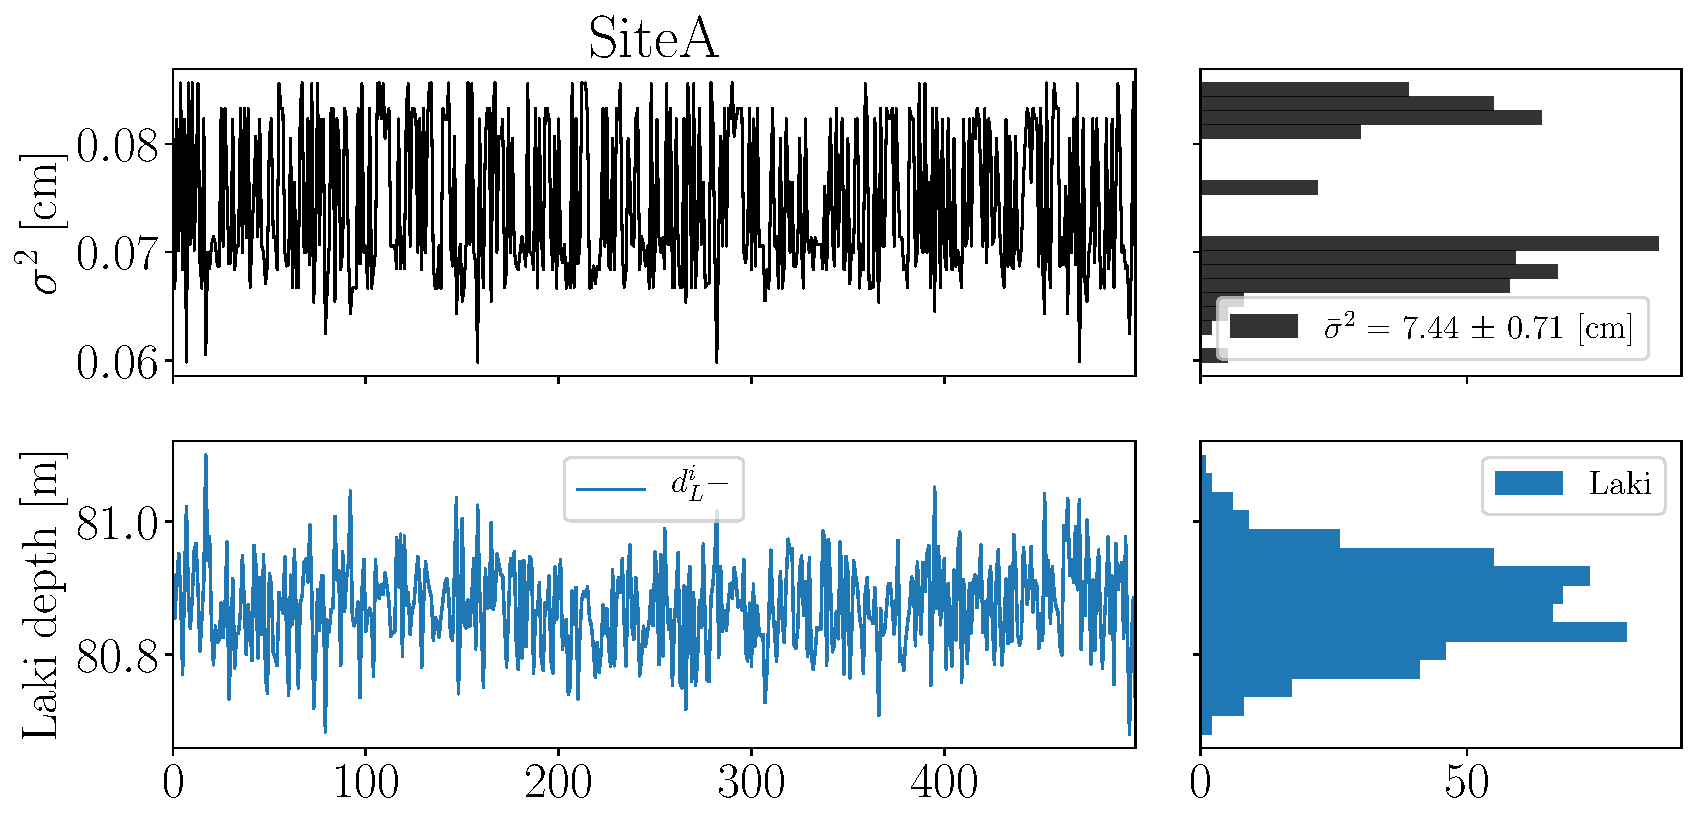
\includegraphics[width=0.95\textwidth]{SiteA_Vary_Lonly.pdf}
	\caption[$\sigma$ variations, varying only Laki]{\small Diffusion length estimates for Site A when varying only the Laki volcanic event. The locations are drawn from Gaussian distributions as the ones presented in Section \ref{Sec:Data_VolcanicHorizons}. The depth section is kept at a constant length, corresponding to the mean distance value, $\bar{d}_{\text{Laki}}-\bar{d}_{\text{Tambora}}$.}
	\label{fig:SiteA_Vary_Tonly}
\end{figure}

The final method is an investigation of drawing the locations of both Laki and Tambora from distributions with a standard deviation of what corresponds to two months and a mean value of where the middle of the volcanic event is estimated to be. An illustration of how much this is in depth is shown in Figure \ref{fig:SiteA_LandT_Gauss_2Mnth}. The results can be seen in Figure \ref{fig:SiteA_LandT_Gauss_2mnth_NDCT}. Again, the possible effect of the quantized grid search can be seen.

%\subsubsection[Vary L]{Varying only Laki Position}
%\label{Subsubsec:Method_TestStab_LTlocations_L}

\begin{figure}[!h]
	\centering
	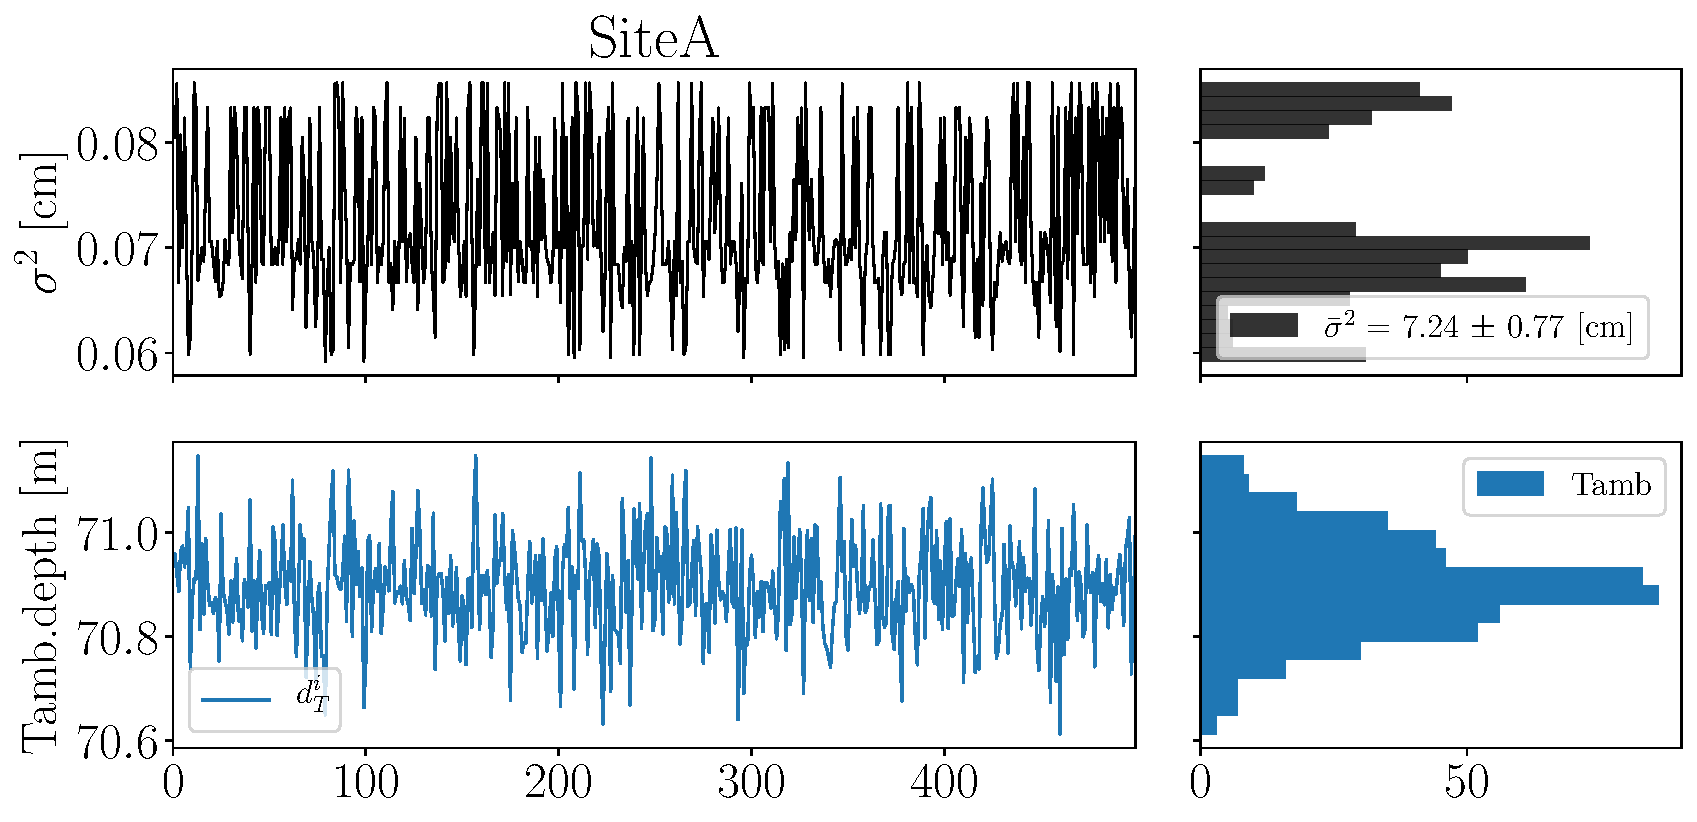
\includegraphics[width=0.95\textwidth]{SiteA_Vary_Tonly.pdf}
	\caption[$\sigma$ variations, varying only Tambora]{\small Diffusion length estimates for Site A when varying only the Tambora volcanic event. The locations are drawn from Gaussian distributions as the ones presented in Section \ref{Sec:Data_VolcanicHorizons}. The depth section is kept at a constant length, corresponding to the mean distance value, $\bar{d}_{\text{Laki}}-\bar{d}_{\text{Tambora}}$.}
	\label{fig:SiteA_Vary_Lonly}
\end{figure}



%\subsubsection[2 Month Variability]{Variation Corresponding to 2 Months}
%\label{Subsubsec:Method_TestStab_LTlocations_2Month}

\begin{figure}[!h]
	\centering
	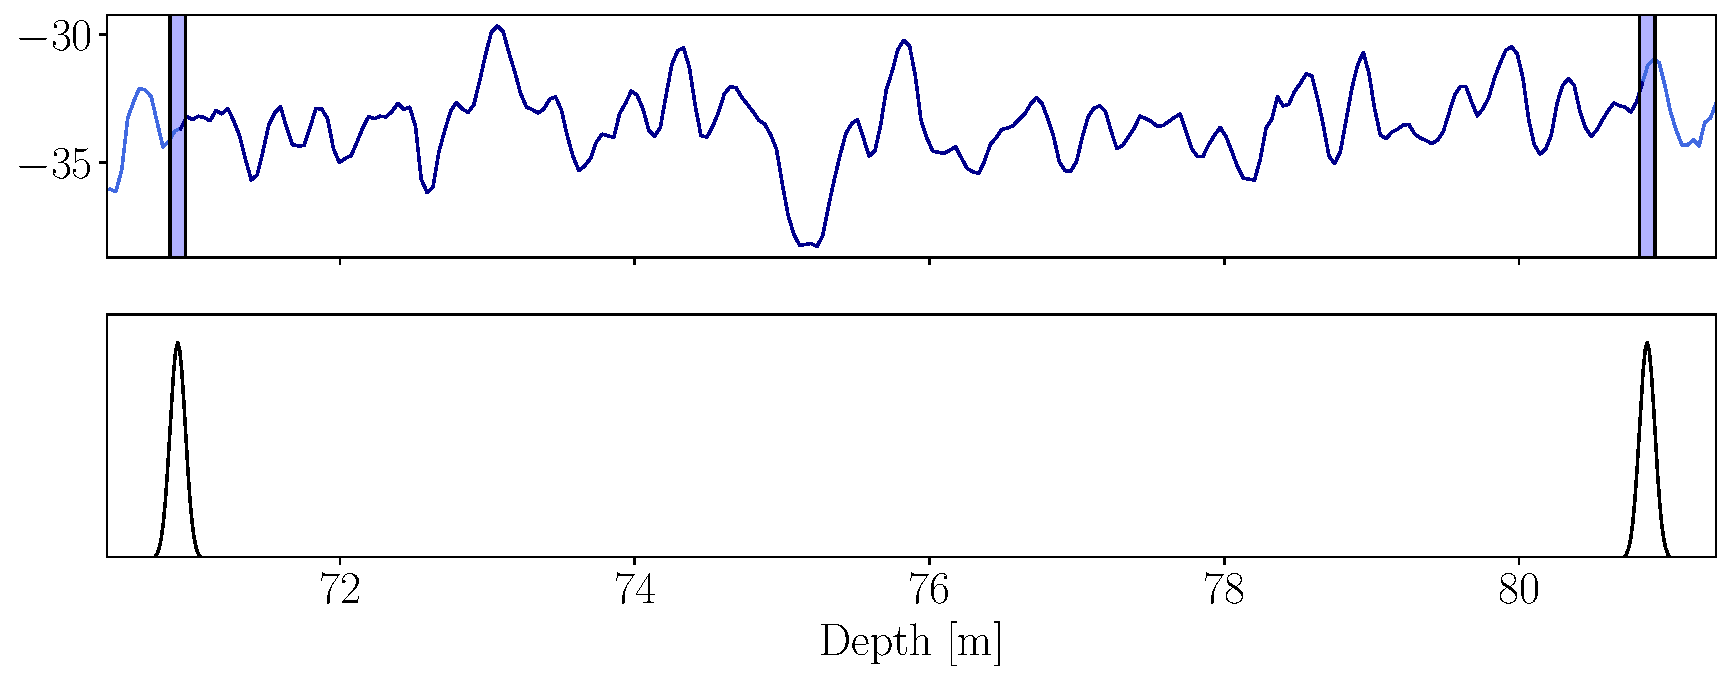
\includegraphics[width=0.95\textwidth]{SiteA_LandT_Gauss_2Mnth.pdf}
	\caption[2 month st. dev. variation of volcanic events locations]{\small Illustration of the method implemented to manage the uncertainty of the exact depth location of the volcanic events. The method establishes a Gaussian distribution with a mean of the estimated middle of the volcanic event and a standard deviation of what corresponds to two months.}
	\label{fig:SiteA_LandT_Gauss_2Mnth}
\end{figure}

%\begin{figure}[h]
%	\centering
%	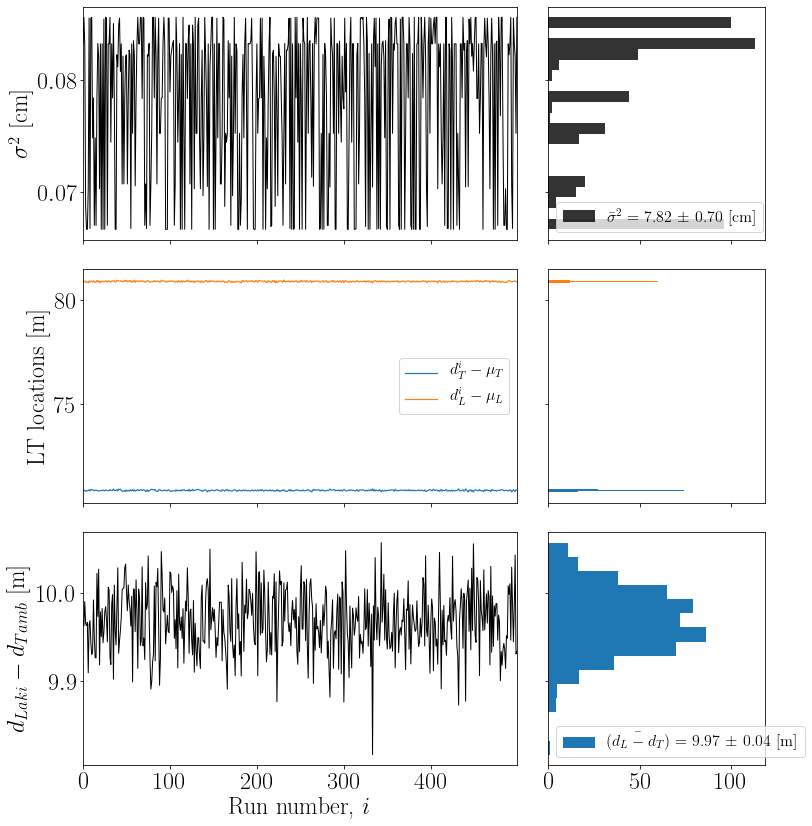
\includegraphics[width=0.95\textwidth]{SiteA_Vary_LandT_2mnth_DCT.png}
%	\caption[2 Month Variation of Event Locations, Site A]{\small 500 runs with locations of Laki and Tambora events drawn from a Gaussian distribution with a standard deviation of two months. Using DCT as spectral transform.}
%	\label{fig:SiteA_LandT_Gauss_2mnth_DCT}
%\end{figure}

\begin{figure}[!htb]
	\centering
	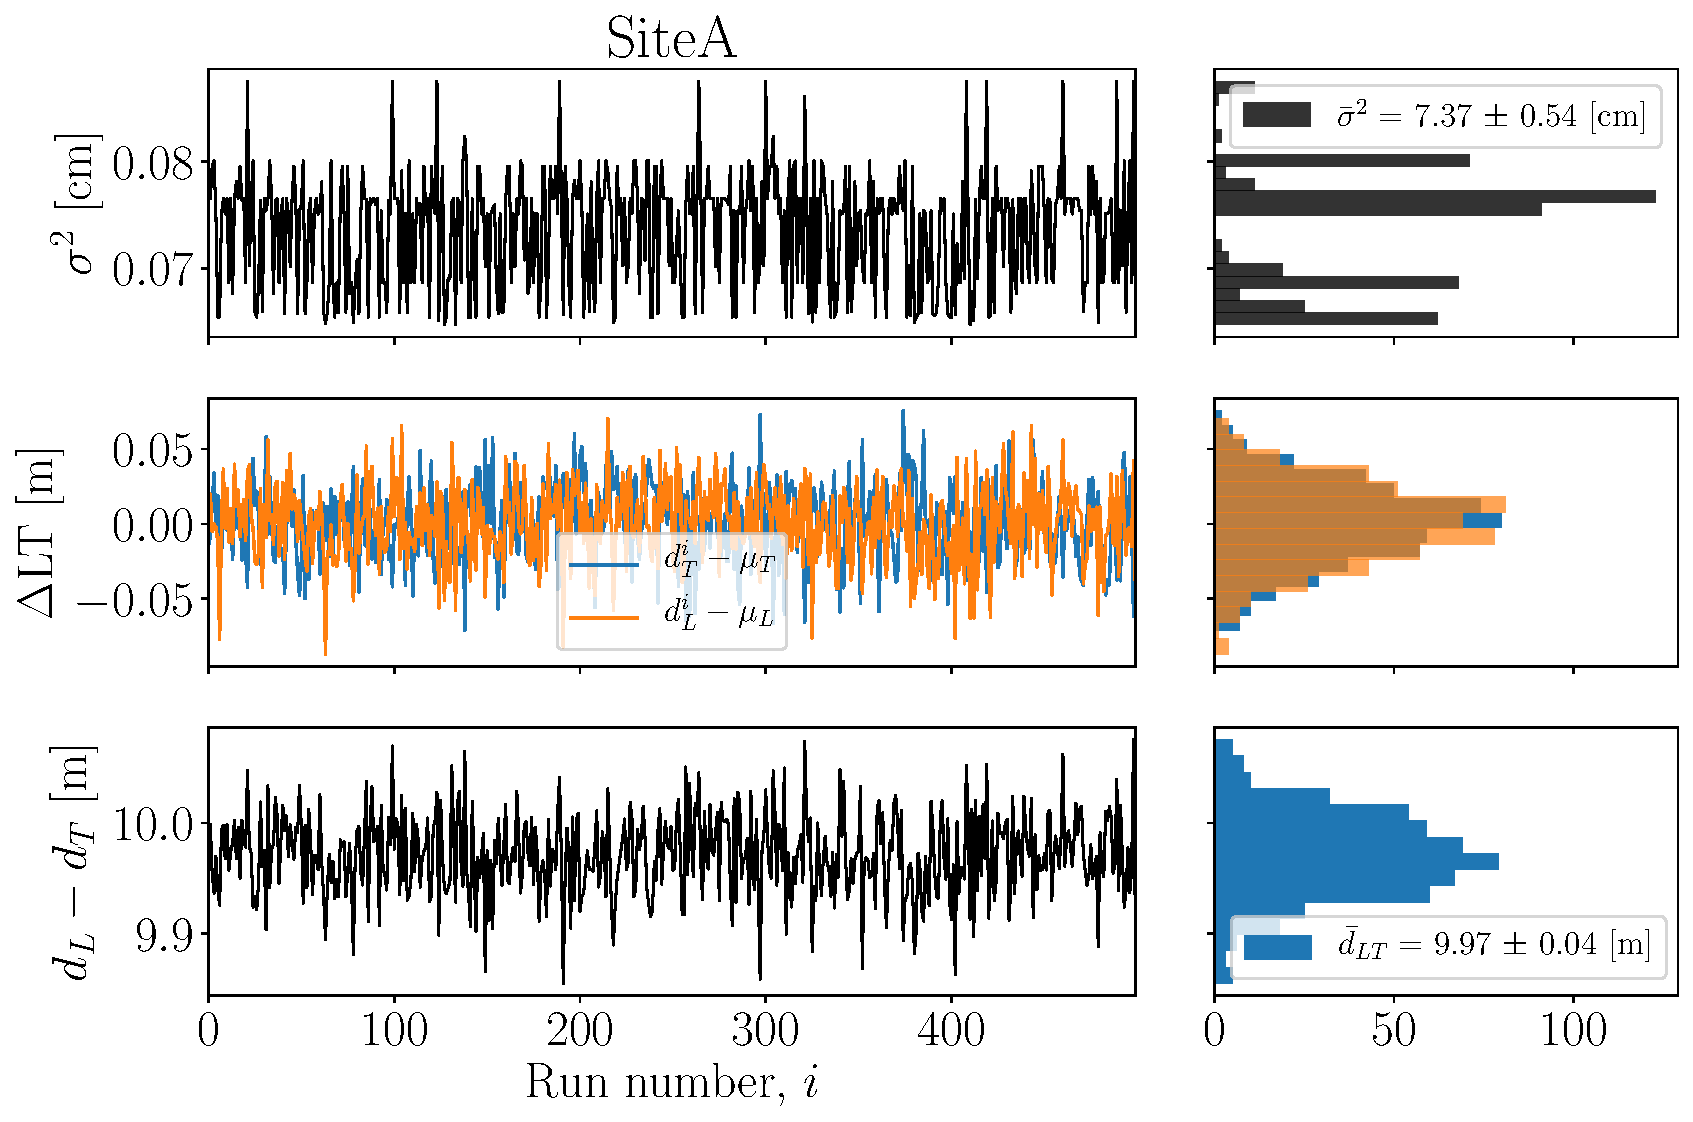
\includegraphics[width=0.95\textwidth]{SiteA_Vary_LandT_2mnth_NDCT.pdf}
	\caption[2 month variation of event locations, Site A]{\small 500 runs with locations of Laki and Tambora events drawn from a Gaussian distribution with a standard deviation of two months, using NDCT as spectral transform.}
	\label{fig:SiteA_LandT_Gauss_2mnth_NDCT}
\end{figure}



\section[Upgrades][Upgrades]{Possible Algorithm Upgrades}
\label{Sec:Method_Upgrades}
In future work, a number of different areas in the method and the algorithm could be upgraded and continuously developed. Some of these further work points will be presented and discussed here.

The peak detection method in the optimization module is, as mentioned, very simply developed. There are ways that this method could be improved, for example by taking the entire yearly pattern of winter(peak)-spring-summer(trough)-fall (PSTF) into account when detecting the pattern. This could possibly be done by investigating the derivative in the signal, and assigning S and F values to the steepest part between a P and a T. There is also a possibility to develop a more sophisticated and maybe intelligent pattern recognition algorithm to detect yearly cycles in the signals. The pattern recognition could be based on the undiffused isotopic signals in the shallower parts of different ice cores. This would improve the certainty of detecting the right number of years in the section. By implementing more seasons, it also allows for more precise dating.

Considering the optimization routine, some issues have already presented themselves, through the distributions of the final results. These quantizations of the final results might be an effect of the search method, and could maybe be avoided by introducing a factor of randomness into the grid search. Furthermore, when shifting the estimated volcanic event positions to generate uncertainties, the optimization should also take into account if the constraints should be changed. If the locations add or subtract length from the signal, the number of peaks and troughs should also be considered to be raised or lowered. This could be worked in with the more detailed pattern recognition.

The frequency filter construction could also be investigated further. It might be allowing too much noise, or filtering some cycles away that were actually interesting. The construction could be made variable and work with the optimization module to tune and change as the constraints do. Some of these issues could be dealt with by gaining a higher resolution from the data by increasing the sampling rate in future measurements - interpolation can only get us so far without a large risk of misinterpretation. 

This work has focused on estimating the maximal diffusion length that fulfills the imposed constraints. Another focus point could be on investigating all $\sigma$ that fulfill the constraints. This could give a temperature range estimate instead of just one temperature estimate. Furthermore, the stability of the method at a given section might be investigated through this as well, as a section that only allows for a very limited $\sigma$ range might actually show that the imposed constraints are not valid.


Furthermore, an in depth investigation and implementation of working with a variable diffusion length, $\sigma(z)$, instead of a constant $\sigma_{\text{const}}$ could present a more accurate estimate of the final $\sigma_{\text{Opt}}(z)$ for the entire depth section, and not just an average. If this was implemented further, it might allow for a more thorough analysis of the variation in temperature in the depth section, instead of only examining the mean temperature of the time frame. Implementing $\sigma(z)$ could also allow for a better estimate of $\sigma_{\text{firn}}$, if the samples are unevenly sampled, as the firn diffusion length estimate then could be made individually point by point based on both sample size and diffusion length estimate at that point.

%\subsection[Peak Detection]{Peak Detection}
%\label{Subsec:Method_Upgrades_PeakDet}
%
%\subsection[Optimization Routine]{Optimization Routine}
%\label{Subsec:Method_Upgrades_OptiRout}









\end{document}
